\documentclass{article}

\usepackage{arxiv}

\usepackage[utf8]{inputenc} % allow utf-8 input
\usepackage[T1]{fontenc}    % use 8-bit T1 fonts
\usepackage{lmodern}        % https://github.com/rstudio/rticles/issues/343
\usepackage{hyperref}       % hyperlinks
\usepackage{url}            % simple URL typesetting
\usepackage{booktabs}       % professional-quality tables
\usepackage{amsfonts}       % blackboard math symbols
\usepackage{nicefrac}       % compact symbols for 1/2, etc.
\usepackage{microtype}      % microtypography
\usepackage{graphicx}

\title{cubble An R Package for Structuring Spatio-temporal Data}

\author{
    H. Sherry Zhang
   \\
    Monash University \\
  21 Chancellors Walk, Clayton VIC 3800 Australia \\
  \texttt{\href{mailto:huize.zhang@monash.edu}{\nolinkurl{huize.zhang@monash.edu}}} \\
   \And
    Dianne Cook
   \\
    Monash University \\
  21 Chancellors Walk, Clayton VIC 3800 Australia \\
  \texttt{\href{mailto:dicook@monash.edu}{\nolinkurl{dicook@monash.edu}}} \\
   \And
    Ursula Laa
   \\
    University of Natural Resources and Life Sciences \\
  Gregor-Mendel-Straße 33, 1180 Wien, Austria \\
  \texttt{\href{mailto:ursula.laa@boku.ac.at}{\nolinkurl{ursula.laa@boku.ac.at}}} \\
   \And
    Nicolas Langrené
   \\
    BNU-HKBU United International College \\
  2000 Jintong Road, Tangjiawan, Zhuhai, Guangdong Province, China \\
  \texttt{\href{mailto:nicolaslangrene@uic.edu.cn}{\nolinkurl{nicolaslangrene@uic.edu.cn}}} \\
   \And
    Patricia Menéndez
   \\
    Monash University \\
  21 Chancellors Walk, Clayton VIC 3800 Australia \\
  \texttt{\href{mailto:patricia.menendez@monash.edu}{\nolinkurl{patricia.menendez@monash.edu}}} \\
  }

% Pandoc syntax highlighting
\usepackage{color}
\usepackage{fancyvrb}
\newcommand{\VerbBar}{|}
\newcommand{\VERB}{\Verb[commandchars=\\\{\}]}
\DefineVerbatimEnvironment{Highlighting}{Verbatim}{commandchars=\\\{\}}
% Add ',fontsize=\small' for more characters per line
\usepackage{framed}
\definecolor{shadecolor}{RGB}{248,248,248}
\newenvironment{Shaded}{\begin{snugshade}}{\end{snugshade}}
\newcommand{\AlertTok}[1]{\textcolor[rgb]{0.94,0.16,0.16}{#1}}
\newcommand{\AnnotationTok}[1]{\textcolor[rgb]{0.56,0.35,0.01}{\textbf{\textit{#1}}}}
\newcommand{\AttributeTok}[1]{\textcolor[rgb]{0.77,0.63,0.00}{#1}}
\newcommand{\BaseNTok}[1]{\textcolor[rgb]{0.00,0.00,0.81}{#1}}
\newcommand{\BuiltInTok}[1]{#1}
\newcommand{\CharTok}[1]{\textcolor[rgb]{0.31,0.60,0.02}{#1}}
\newcommand{\CommentTok}[1]{\textcolor[rgb]{0.56,0.35,0.01}{\textit{#1}}}
\newcommand{\CommentVarTok}[1]{\textcolor[rgb]{0.56,0.35,0.01}{\textbf{\textit{#1}}}}
\newcommand{\ConstantTok}[1]{\textcolor[rgb]{0.00,0.00,0.00}{#1}}
\newcommand{\ControlFlowTok}[1]{\textcolor[rgb]{0.13,0.29,0.53}{\textbf{#1}}}
\newcommand{\DataTypeTok}[1]{\textcolor[rgb]{0.13,0.29,0.53}{#1}}
\newcommand{\DecValTok}[1]{\textcolor[rgb]{0.00,0.00,0.81}{#1}}
\newcommand{\DocumentationTok}[1]{\textcolor[rgb]{0.56,0.35,0.01}{\textbf{\textit{#1}}}}
\newcommand{\ErrorTok}[1]{\textcolor[rgb]{0.64,0.00,0.00}{\textbf{#1}}}
\newcommand{\ExtensionTok}[1]{#1}
\newcommand{\FloatTok}[1]{\textcolor[rgb]{0.00,0.00,0.81}{#1}}
\newcommand{\FunctionTok}[1]{\textcolor[rgb]{0.00,0.00,0.00}{#1}}
\newcommand{\ImportTok}[1]{#1}
\newcommand{\InformationTok}[1]{\textcolor[rgb]{0.56,0.35,0.01}{\textbf{\textit{#1}}}}
\newcommand{\KeywordTok}[1]{\textcolor[rgb]{0.13,0.29,0.53}{\textbf{#1}}}
\newcommand{\NormalTok}[1]{#1}
\newcommand{\OperatorTok}[1]{\textcolor[rgb]{0.81,0.36,0.00}{\textbf{#1}}}
\newcommand{\OtherTok}[1]{\textcolor[rgb]{0.56,0.35,0.01}{#1}}
\newcommand{\PreprocessorTok}[1]{\textcolor[rgb]{0.56,0.35,0.01}{\textit{#1}}}
\newcommand{\RegionMarkerTok}[1]{#1}
\newcommand{\SpecialCharTok}[1]{\textcolor[rgb]{0.00,0.00,0.00}{#1}}
\newcommand{\SpecialStringTok}[1]{\textcolor[rgb]{0.31,0.60,0.02}{#1}}
\newcommand{\StringTok}[1]{\textcolor[rgb]{0.31,0.60,0.02}{#1}}
\newcommand{\VariableTok}[1]{\textcolor[rgb]{0.00,0.00,0.00}{#1}}
\newcommand{\VerbatimStringTok}[1]{\textcolor[rgb]{0.31,0.60,0.02}{#1}}
\newcommand{\WarningTok}[1]{\textcolor[rgb]{0.56,0.35,0.01}{\textbf{\textit{#1}}}}

% tightlist command for lists without linebreak
\providecommand{\tightlist}{%
  \setlength{\itemsep}{0pt}\setlength{\parskip}{0pt}}


% Pandoc citation processing
\newlength{\cslhangindent}
\setlength{\cslhangindent}{1.5em}
\newlength{\csllabelwidth}
\setlength{\csllabelwidth}{3em}
\newlength{\cslentryspacingunit} % times entry-spacing
\setlength{\cslentryspacingunit}{\parskip}
% for Pandoc 2.8 to 2.10.1
\newenvironment{cslreferences}%
  {}%
  {\par}
% For Pandoc 2.11+
\newenvironment{CSLReferences}[2] % #1 hanging-ident, #2 entry spacing
 {% don't indent paragraphs
  \setlength{\parindent}{0pt}
  % turn on hanging indent if param 1 is 1
  \ifodd #1
  \let\oldpar\par
  \def\par{\hangindent=\cslhangindent\oldpar}
  \fi
  % set entry spacing
  \setlength{\parskip}{#2\cslentryspacingunit}
 }%
 {}
\usepackage{calc}
\newcommand{\CSLBlock}[1]{#1\hfill\break}
\newcommand{\CSLLeftMargin}[1]{\parbox[t]{\csllabelwidth}{#1}}
\newcommand{\CSLRightInline}[1]{\parbox[t]{\linewidth - \csllabelwidth}{#1}\break}
\newcommand{\CSLIndent}[1]{\hspace{\cslhangindent}#1}

\begin{document}
\maketitle


\begin{abstract}
Spatio-temporal data refer to measurements taken across space and time.
In practice, spatio-temporal data can be decomposed into a spatial and
temporal component: at one time, we would select a spatial location and
inspect the temporal trend; at other time, we might select one or
multiple time value(s) and explore the spatial distribution. Ideally, we
could make multiple maps and multiple time series to explore these
together, however, doing all of these actions is complicated when data
arrive fragmented in multiple objects. To make it easy to do all these
tasks, ideally spatial and temporal variables are in a single data
object that we can slice and dice in different ways to conduct different
visualisations. This work suggests a new data structure, \code{cubble},
that uses a nested form and a long form to organise spatial and temporal
variables in a single data object. The new data structure ensures that
data in the two forms are synchronised while been flexible to explore
the two aspect of spatio-temporal data. It also provides capability for
handling data with hierarchical structure, matching data from multiple
sources, constructing interactive graphics, and performing
spatio-temporal transformation. The paper will demonstrate \pkg{cubble}
with examples using Australian climate weather stations, river level
data, and climate reanalysis (ERA5) data.
\end{abstract}

\keywords{
    spatial, temporal, spatio temporal, R, environmental data,
    exploratory data analysis
  }

\newpage

\hypertarget{introduction}{%
\section{Introduction}\label{introduction}}

Spatio-temporal data involves variables observed in the space across
time and this paper focuses on spatio-temporal vector data with fixed
locations and regular time intervals. This type of data can naturally be
considered as a data cube with three axes: spatial identifier, temporal
identifier, and variables. In this cubic formation, space only occupies
one axis, rather than two, to avoid hypercubes for multivariate
spatio-temporal data. While conceptually the data format is relatively
simple, the data objects coming to the analysts can vary in forms in the
analysis. Figure \ref{fig:illu-input} shows three examples of wild
spatio-temporal data: 1) a single table that includes both the spatial
and temporal variables; 2) separate tables for spatial and temporal
variables; 3) array-based data, i.e.~NetCDF (Network Common Data Form)
data, which is commonly used in earth science, e.g.~climatology,
meteorology, and oceanography, among others, to organise multivariate
data in a spatio-temporal grid.

\begin{figure}

{\centering 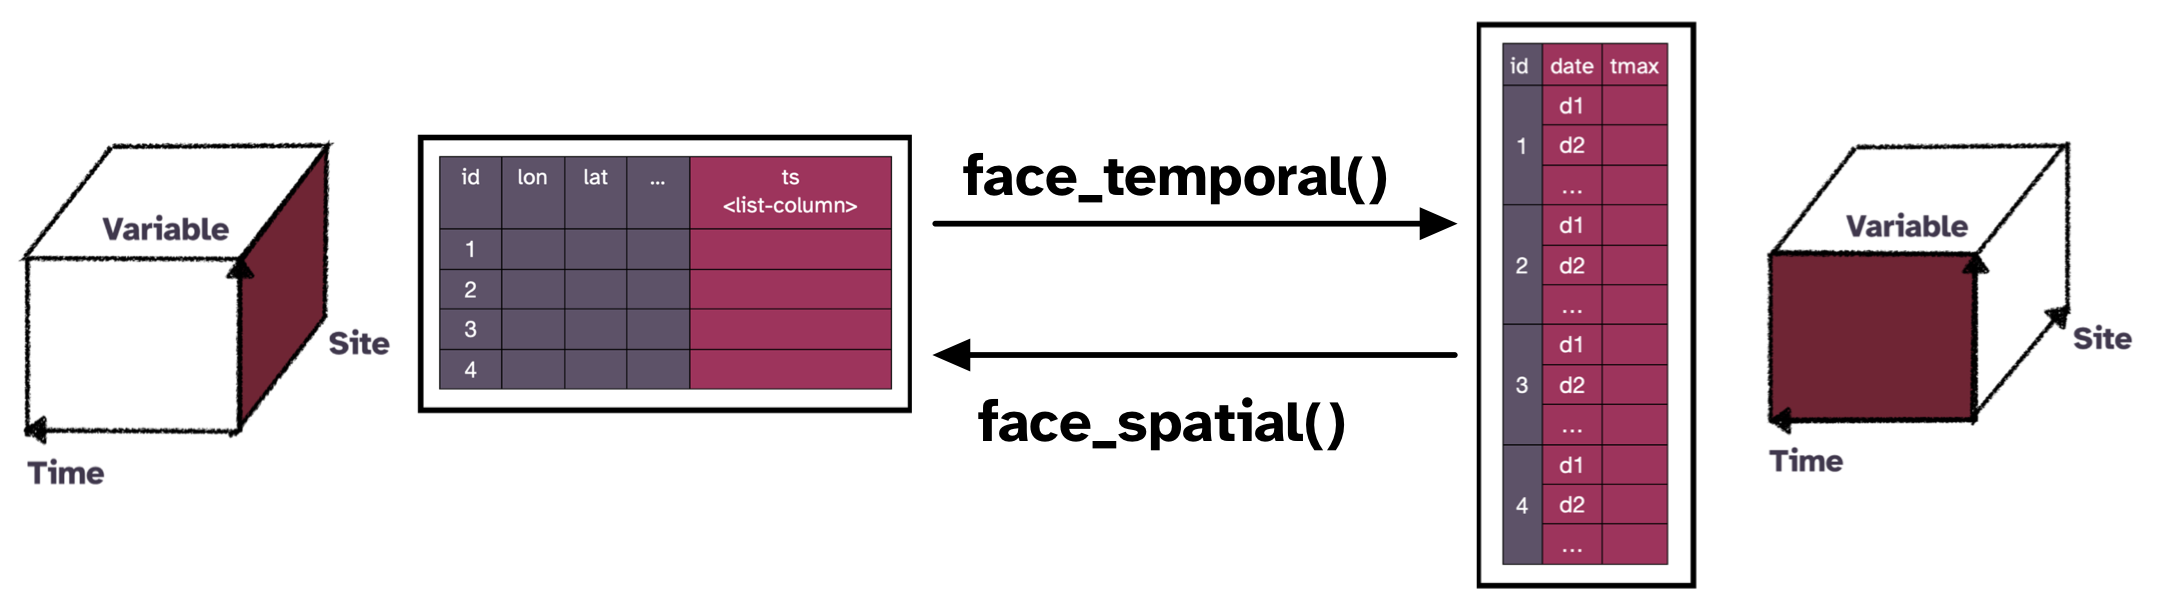
\includegraphics[width=1\linewidth]{/Users/sherryzhang/Documents/research/paper-cubble/figures/diagram-keynotes/diagram-keynotes.001} 

}

\caption{An illustration of different spatio-temporal data layouts: (1) a single table for both spatial and temporal variables; (2) separate tables for spatial and temporal variables; and (3) an array data structure that populates variables into a gridded longitude-latitude-time (hyper)cube.}\label{fig:illu-input}
\end{figure}

While incorporating both spatial and temporal information enriches the
data in the analysis, spatio-temporal data can sometimes be hard to work
with given its two observational units in the variables. The single
table format in Figure \ref{fig:illu-input} is convenient for
spatio-temporal operations that involve both types of variables,
however, it makes duplicates of spatial variables and is not ideal when
only looking at the spatial aspect of the data. The two tables format
allows separate operations on spatial and temporal variables while
analysts need to work with two data objects simultaneously and join them
together into the single table format for spatio-temporal operations.
Neither of the two formats is desirable at the same time for spatial,
temporal, and spatio-temporal operations. This issue implies analysts
need to constantly think about the data format and arrange variables
into the proper shape before the actual operations, which can be a
laborious step when switching between the two formats back and forth
several times during the analysis.

In the \proglang{R} community, many data objects have been proposed to
work with specific spatio-temporal tasks, while few can freely explore
the data. \pkg{spacetime} (\protect\hyperlink{ref-spacetime}{E. Pebesma
2012}) is an attempt for such a data object, but the spatial and
temporal classes it is built on have now been gradually replaced by more
recent implementations. The \pkg{stars}
(\protect\hyperlink{ref-stars}{E. Pebesma 2021}) package uses an array
to wrangle spatio-temporal data, but the dense array it uses can quickly
exhaust the memory for data in the case of irregular spatial grid. While
there has not yet been a data object that makes it easy to wrangle
spatio-temporal data, there is a strong need for such tools given the
ubiquitous spatial and temporal data collected in the society, i.e.,
climate observations from weather stations, air quality variables from
air monitoring stations. The demand for such tools can also come from
spatial data analysts wishing to incorporate temporal data in their
analysis or vice versa.

This paper presents a new \proglang{R} package, \pkg{cubble}, to
overcome the problem with organising variables in different levels when
working with spatio-temporal data. In the package a new data structure,
also called \code{cubble}, is proposed to organise spatial and temporal
variables as two forms of a single data object so that they can be
wrangled separately while synchronised as a whole piece. With this new
data object, analysts can spend less time writing codes to organise
spatial and temporal variables and focus more on the exploratory data
analysis itself. The software is available from the Comprehensive R
Archive Network (CRAN) at {[}CRAN link{]}.

The rest of the paper is divided as follows: Section 2 presents the main
design and functionality of \pkg{cubble}. Section 3 explains how cubble
deals with more advanced considerations including data with hierarchical
structure, data matching, how cubble fits with existing static and
interactive visualisation tools, and spatio-temporal data
transformation. Section 4 uses Australia weather station data and river
level data as examples to demonstrate the use of \pkg{cubble}. An
example on how \pkg{cubble} handles NetCDF data is also provided.
Section 5 concludes the paper.

\hypertarget{conceptual-framework-spatio-temporal-cube}{%
\section{Conceptual framework: spatio-temporal
cube}\label{conceptual-framework-spatio-temporal-cube}}

Multivariate spatio-temporal data can be conceptualised using a cubical
data model with reference to variables, time and space. This naturally
motivates the usage of array to represent and store spatio-temporal
data, as evident by satellite imageries, large climate models, among
others. The work by Lu, Appel, and Pebesma
(\protect\hyperlink{ref-lu_multidimensional_2018}{2018}) has discussed
the suitability of this representation through array algebra and
practical spatio-temporal tasks.

The cubical conceptual framework provides a generalisation to the
operation can be done on the data for visualisation. A paper by Bach et
al. (\protect\hyperlink{ref-bach_review_2014}{2014}) has reviewed the
temporal data visualisation based on space-time cube operations. Notice
that the term space-time cube in their article ``does not need to
involve spatial data'', but referring to ``an abstract 2D substrate that
is used to visualize data at a specific time''. Despite its main focus
is on temporal data, the mindset of abstracting out data representation
to construct visualisation is applicable to our spatio-temporal data
manipulation and visualisation.

\hypertarget{existing-work-and-new-challenges}{%
\section{Existing work and new
challenges}\label{existing-work-and-new-challenges}}

To represent spatio-temporal data, E. Pebesma
(\protect\hyperlink{ref-spacetime}{2012}) proposes four layouts: full
grid layout (STF), sparse grid layout (STS), irregular layout (STI), and
trajectory (STT). These layouts are implemented in the \pkg{spacetime}
package with underlying class \pkg{sp} (\protect\hyperlink{ref-sp}{E.
Pebesma and Bivand 2005}) and \pkg{xts}
(\protect\hyperlink{ref-xts}{Ryan and Ulrich 2020}) for handling spatial
and temporal variables. While these layouts and classes are still being
used and well-maintained today, they are not compatible with the
\pkg{tidyverse} ecosystem (\protect\hyperlink{ref-tidyverse}{Wickham et
al. 2019}), which has a huge influence on data analysis in \proglang{R},
including in the spatial and temporal communities. The package \pkg{sf}
(\protect\hyperlink{ref-sf}{E. J. Pebesma 2018}) uses data frame objects
to represent spatial data with an additional \code{geometry} column
dedicating to feature geometries
(\protect\hyperlink{ref-jr_herring_opengis_2011}{J.R. Herring 2011})
(e.g.~POINT, MULTIPOINT, POLYGON, MULTIPOLYGON etc). For temporal data,
\pkg{tsibble} (\protect\hyperlink{ref-tsibble}{Wang, Cook, and Hyndman
2020a}) builds on top of the \pkg{tibble}
(\protect\hyperlink{ref-tibble}{Müller and Wickham 2021}) object and
explicitly includes date and time in columns as variables, rather than
data attributes.

Underlying tidyverse is the concept of tidy data
(\protect\hyperlink{ref-tidydata}{Wickham 2014}), which considers how
variables should be structured for analysis. In the three formats
(time-wide, space-wide, and long) summarised in the E. Pebesma
(\protect\hyperlink{ref-spacetime}{2012}) paper, only the long form is
considered as tidy. The main advantages of it over the time-wide and
space-wide format is that the latter treat either time or location as
variable names (Section 3.1 in Wickham
(\protect\hyperlink{ref-tidydata}{2014})) rather than values of
variables, making them difficult to be wrangled. One problem with the
long format is that it can be inefficient to store feature geometries,
especially for large MULTIPOLYGON over long time period. This motivates
a new tidyverse compatible data object to work with spatio-temporal
data.

\textbf{two challenages: multiple data sources + large spatio-temporal
object} In additional to the shift into more tidyverse workflow for
working with data, spatio-temporal data have some unique challenges. The
first one being the split of variables in multiple tables. Often the
time, spatio-temporal data is not presented in a single data object, but
split into fragmented pieces from different sources. For example, map
data recorded the shape of a collection of area of interest is provided
by the government website; the geo-scientific data is recorded with
longitude and latitude coordinate of locations in the area; and temporal
variables indexed by both location and time need to be further queried
using location data. For spatio-temporal data analysis, merging all
these sources can be challenging and joining these tables can go wrong
because of the slightest unmatched of the linking variable from
different sources.

Another challenge when analysing spatio-temporal data is on the simple
feature representation of spatial data. While the simple feature is able
to handle large and complex spatial geometry and perform precise spatial
operations, data analysts usually do not have a large expectation on the
map accuracy and would prefer a simplified map with quick rendering for
visualisation. Also, the feature geometry column in \pkg{sf} wraps the
spatial coordinates in a list column, sometimes, analysts may like to
unpack them into longitude and latitude to work with. A smooth
transition with the coordinate columns and and simple feature geometry
column would satisfy analysts from both ends.

With some of the aforementioned issues recognised, the \pkg{stars}
package has been a new implementation to handle spatio-temporal data
conceptually as data cubes and implemented as arrays. The package
depends on the \pkg{sf} package and has allowed more access to tidyverse
verbs in the workflow. However, for vector spatio-temporal data, major
difficulties to work with \pkg{stars} is first to cast the variables
from multiple tables into a star object and then keep the operations in
the high-dimensional cube. Given that most table mentioned before
collect variables in a 2D table, analysts could benefit from a structure
to allow them work in 2D tables.

\hypertarget{the-cubble-package}{%
\section{The cubble package}\label{the-cubble-package}}

This section will present two formats that cubble uses to arrange
spatio-temporal data. The main cubble functions will then be introduced
to illustrate how to work with these two formats in short examples.
Lastly, a subsection will be dedicated to how existing packages, in
spatial and temporal analysis, fit in with cubble.

In cubble, a single data object can be arranged into two forms: nested
form and long form. Figure \ref{fig:illu-cubble} sketches the two forms
with the associated attributes. The decision on which form to use in
data wrangling is output-oriented, meaning analysts need to first think
about whether the output of an operation is identified only by the
spatial identifier, or a combination of spatial and temporal identifier.
The nested cubble is suitable for working with operations that are only
identified by the site and this type of operation can be a pure
manipulation of time invariant variables, or an operation that
summarises time varying variables into site. Underneath the nested form,
a cubble is built from a \code{rowwise_df} class where each site forms a
separate group. This structure simplifies the calculation that involves
temporal variables by avoiding the use of \code{purrr::map()} syntax
when working with list-column.

For those operations whose output involves both a spatial and temporal
identifier, long form should be used. The long form uses a
\code{grouped_df} class to forms all the time of a site as a group. Time
invariant variables are stored separately as an special attribute of the
long cubble. This design avoids repeating the spatial variables at each
time stamp while not dropping information from spatial variables.

\begin{figure}

{\centering 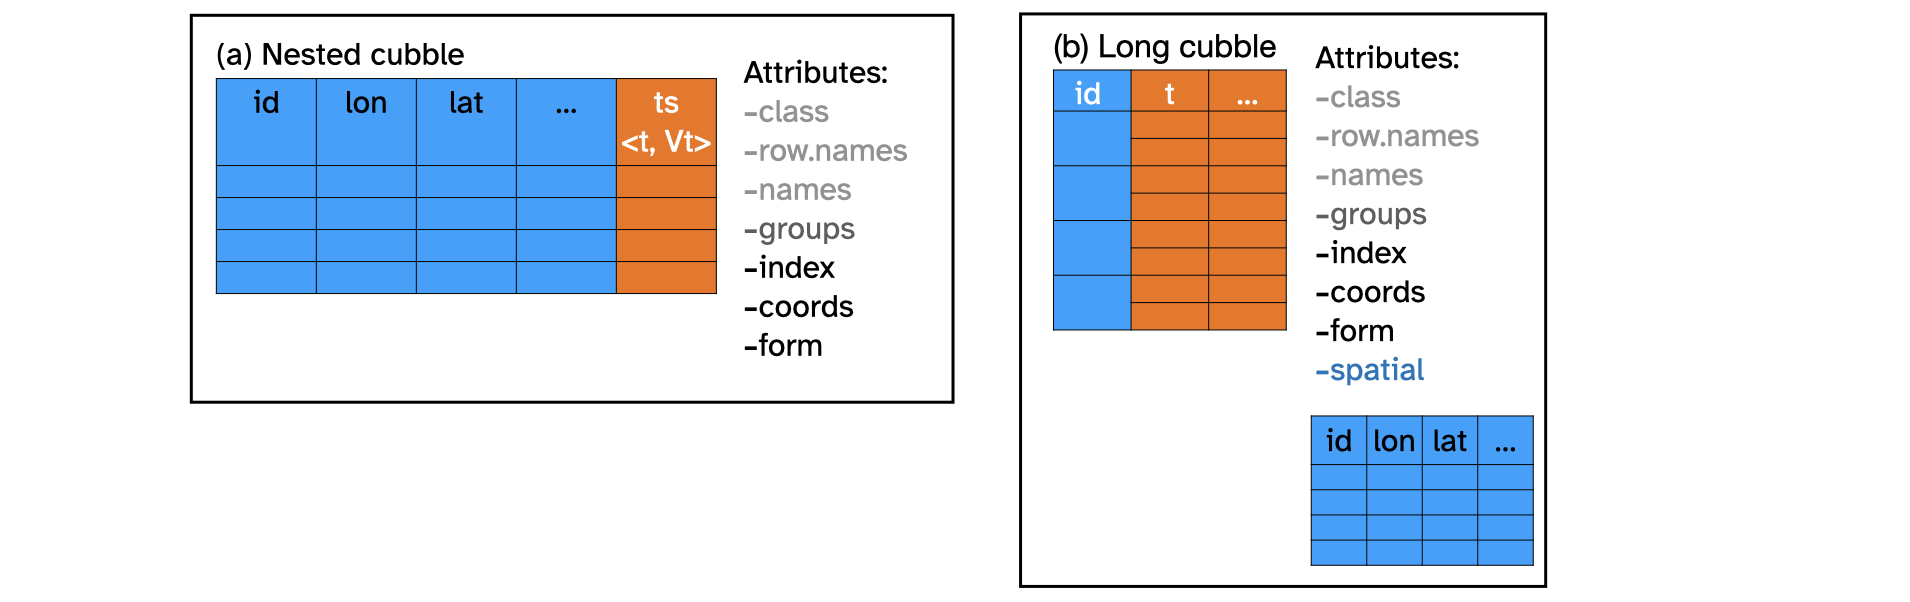
\includegraphics[width=1\linewidth]{/Users/sherryzhang/Documents/research/paper-cubble/figures/diagram-keynotes/diagram-keynotes.002} 

}

\caption{An illustration of the nested and long form in cubble. The nested form defines each site in a row and nests the time varying variables into a single column \code{ts}. The long form cubble uses \code{id} and \code{t} to identify each row and stores the time invariant variables as an attribute, \code{spatial}.}\label{fig:illu-cubble}
\end{figure}

\hypertarget{create-a-cubble-in-the-nested-form}{%
\subsection{Create a cubble in the nested
form}\label{create-a-cubble-in-the-nested-form}}

To use functions in the \texttt{cubble} package, an analyst will first
need to turn the data object into a \code{cubble} class.
\code{as_cubble()} does this through supplying the three key components:
\code{key} as the spatial identifier; \code{index} as the temporal
identifier; and a vector of \code{coords} in the order of longitude and
latitude. The use of \code{key} and \code{index} follows the design in
the \pkg{tsibble} package and the cubble created by default is in the
nested form.

Before the formal examples in Section \ref{examples}, each function
introduced in this section will be accompanied by a small example. The
data used for the small examples is a subset of a larger climate weather
station data used in the formal examples and has been simplified to
include only five weather stations. It contains spatial information of
each station: station id, latitude, longitude, elevation, station name
and World Meteorology Organisation ID and also daily temporal
information of date, maximum and minimum temperature and precipitation
for 2020. \code{climate_flat} stores this data in format 1) in Figure
\ref{fig:illu-input} and the code below creates a cubble out of
\code{climate_flat} with \code{id} as the key, \code{date} as the index,
and \code{c(long, lat)} as the coordinates:

\begin{Shaded}
\begin{Highlighting}[]
\NormalTok{cubble\_nested }\OtherTok{\textless{}{-}}\NormalTok{ cubble}\SpecialCharTok{::}\NormalTok{climate\_flat }\SpecialCharTok{|}\ErrorTok{\textgreater{}}
  \FunctionTok{as\_cubble}\NormalTok{(}\AttributeTok{key =}\NormalTok{ id, }\AttributeTok{index =}\NormalTok{ date, }\AttributeTok{coords =} \FunctionTok{c}\NormalTok{(long, lat))}
\NormalTok{cubble\_nested}
\end{Highlighting}
\end{Shaded}

\begin{verbatim}
## # cubble:   id [5]: nested form
## # bbox:     [115.97, -32.94, 133.55, -12.42]
## # temporal: date [date], prcp [dbl], tmax [dbl], tmin [dbl]
##   id            lat  long  elev name           wmo_id ts                
##   <chr>       <dbl> <dbl> <dbl> <chr>           <dbl> <list>            
## 1 ASN00009021 -31.9  116.  15.4 perth airport   94610 <tibble [366 x 4]>
## 2 ASN00010311 -31.9  117. 179   york            94623 <tibble [366 x 4]>
## 3 ASN00010614 -32.9  117. 338   narrogin        94627 <tibble [366 x 4]>
## 4 ASN00014015 -12.4  131.  30.4 darwin airport  94120 <tibble [366 x 4]>
## 5 ASN00015131 -17.6  134. 220   elliott         94236 <tibble [366 x 4]>
\end{verbatim}

There are a few information in the cubble header: the name of the
\code{key} variable: \code{id} and its unique number: 5, the bounding
box: \code{[115.97, -32.94, 133.55, -12.42]} , and also the name of
variable nested in the \code{ts} column with its type:
\code{date [date], prcp [dbl], tmax [dbl], tmin [dbl]}.

\hypertarget{stretch-a-nested-cubble-into-the-long-form}{%
\subsection{Stretch a nested cubble into the long
form}\label{stretch-a-nested-cubble-into-the-long-form}}

The nested format is convenient for those operations whose output does
not contain a time dimension. For those outputs that are
cross-identified by the spatial and temporal identifier, a long cubble
needs to be used. The function \code{stretch()} is designed to switch
the cubble from the nested form to the long form. This code shows how to
switch the nested cubble just created into its long form:

\begin{Shaded}
\begin{Highlighting}[]
\NormalTok{cubble\_long }\OtherTok{\textless{}{-}}\NormalTok{ cubble\_nested }\SpecialCharTok{|}\ErrorTok{\textgreater{}} \FunctionTok{face\_temporal}\NormalTok{()}
\NormalTok{cubble\_long}
\end{Highlighting}
\end{Shaded}

\begin{verbatim}
## # cubble:  date, id [5]: long form
## # bbox:    [115.97, -32.94, 133.55, -12.42]
## # spatial: lat [dbl], long [dbl], elev [dbl], name [chr], wmo_id [dbl]
##   id          date        prcp  tmax  tmin
##   <chr>       <date>     <dbl> <dbl> <dbl>
## 1 ASN00009021 2020-01-01     0  31.9  15.3
## 2 ASN00009021 2020-01-02     0  24.9  16.4
## 3 ASN00009021 2020-01-03     6  23.2  13  
## 4 ASN00009021 2020-01-04     0  28.4  12.4
## 5 ASN00009021 2020-01-05     0  35.3  11.6
## # ... with 1,825 more rows
\end{verbatim}

Notice that the third line in the header now shows the name and type of
spatial variables:
\code{lat [dbl], long [dbl], elev [dbl], name [chr], wmo_id [dbl]} and
these variables are now stored as a \code{spatial} attribute of the
data:

\begin{Shaded}
\begin{Highlighting}[]
\FunctionTok{attr}\NormalTok{(cubble\_long, }\StringTok{"spatial"}\NormalTok{)}
\end{Highlighting}
\end{Shaded}

\begin{verbatim}
## # A tibble: 5 x 6
##   id            lat  long  elev name           wmo_id
##   <chr>       <dbl> <dbl> <dbl> <chr>           <dbl>
## 1 ASN00009021 -31.9  116.  15.4 perth airport   94610
## 2 ASN00010311 -31.9  117. 179   york            94623
## 3 ASN00010614 -32.9  117. 338   narrogin        94627
## 4 ASN00014015 -12.4  131.  30.4 darwin airport  94120
## 5 ASN00015131 -17.6  134. 220   elliott         94236
\end{verbatim}

\hypertarget{tamp-a-long-cubble-back-to-the-nested-form}{%
\subsection{Tamp a long cubble back to the nested
form}\label{tamp-a-long-cubble-back-to-the-nested-form}}

Manipulation on the spatial and temporal dimension can be an iterative
process and analysts may need to go back and forth between the nested
and long cubble. \code{tamp()}, an inverse of \code{stretch()}, switches
a long cubble to a nested cubble:

\begin{Shaded}
\begin{Highlighting}[]
\NormalTok{cubble\_back }\OtherTok{\textless{}{-}}\NormalTok{ cubble\_long }\SpecialCharTok{|}\ErrorTok{\textgreater{}} \FunctionTok{face\_spatial}\NormalTok{()}
\NormalTok{cubble\_back}
\end{Highlighting}
\end{Shaded}

\begin{verbatim}
## # cubble:   id [5]: nested form
## # bbox:     [115.97, -32.94, 133.55, -12.42]
## # temporal: date [date], prcp [dbl], tmax [dbl], tmin [dbl]
##   id            lat  long  elev name           wmo_id ts                
##   <chr>       <dbl> <dbl> <dbl> <chr>           <dbl> <list>            
## 1 ASN00009021 -31.9  116.  15.4 perth airport   94610 <tibble [366 x 4]>
## 2 ASN00010311 -31.9  117. 179   york            94623 <tibble [366 x 4]>
## 3 ASN00010614 -32.9  117. 338   narrogin        94627 <tibble [366 x 4]>
## 4 ASN00014015 -12.4  131.  30.4 darwin airport  94120 <tibble [366 x 4]>
## 5 ASN00015131 -17.6  134. 220   elliott         94236 <tibble [366 x 4]>
\end{verbatim}

\hypertarget{migrate-spatial-variables-to-a-long-cubble}{%
\subsection{Migrate spatial variables to a long
cubble}\label{migrate-spatial-variables-to-a-long-cubble}}

Sometimes, analysts may need to apply some variable transformation that
involves both the spatial and temporal variable. An example of this is
the transformation of temporal variables into the spatial dimension in
glyph maps (which will be elaborated in section
\ref{st_transformation}). Cubble allows this operation through
\code{unfold()}, which moves the specified spatial variables into the
long cubble:

\begin{Shaded}
\begin{Highlighting}[]
\NormalTok{cubble\_mig }\OtherTok{\textless{}{-}}\NormalTok{ cubble\_long }\SpecialCharTok{|}\ErrorTok{\textgreater{}} \FunctionTok{unfold}\NormalTok{(long, lat)}
\NormalTok{cubble\_mig}
\end{Highlighting}
\end{Shaded}

\begin{verbatim}
## # cubble:  date, id [5]: long form
## # bbox:    [115.97, -32.94, 133.55, -12.42]
## # spatial: lat [dbl], long [dbl], elev [dbl], name [chr], wmo_id [dbl]
##   id          date        prcp  tmax  tmin  long   lat
##   <chr>       <date>     <dbl> <dbl> <dbl> <dbl> <dbl>
## 1 ASN00009021 2020-01-01     0  31.9  15.3  116. -31.9
## 2 ASN00009021 2020-01-02     0  24.9  16.4  116. -31.9
## 3 ASN00009021 2020-01-03     6  23.2  13    116. -31.9
## 4 ASN00009021 2020-01-04     0  28.4  12.4  116. -31.9
## 5 ASN00009021 2020-01-05     0  35.3  11.6  116. -31.9
## # ... with 1,825 more rows
\end{verbatim}

This function should generally be used in the last step of the analysis
since it is a temporary operation, meaning these added spatial variables
are not stored in the long form and will disappear if switched to the
nested form and then switched back:

\begin{Shaded}
\begin{Highlighting}[]
\NormalTok{cubble\_mig }\SpecialCharTok{|}\ErrorTok{\textgreater{}} \FunctionTok{face\_spatial}\NormalTok{() }\SpecialCharTok{|}\ErrorTok{\textgreater{}} \FunctionTok{face\_temporal}\NormalTok{()}
\end{Highlighting}
\end{Shaded}

\begin{verbatim}
## # cubble:  date, id [5]: long form
## # bbox:    [115.97, -32.94, 133.55, -12.42]
## # spatial: lat [dbl], long [dbl], elev [dbl], name [chr], wmo_id [dbl]
##   id          date        prcp  tmax  tmin
##   <chr>       <date>     <dbl> <dbl> <dbl>
## 1 ASN00009021 2020-01-01     0  31.9  15.3
## 2 ASN00009021 2020-01-02     0  24.9  16.4
## 3 ASN00009021 2020-01-03     6  23.2  13  
## 4 ASN00009021 2020-01-04     0  28.4  12.4
## 5 ASN00009021 2020-01-05     0  35.3  11.6
## # ... with 1,825 more rows
\end{verbatim}

\hypertarget{compatibility-with-existing-packages}{%
\subsection{Compatibility with existing
packages}\label{compatibility-with-existing-packages}}

The previous four subsections have introduced operations specific to the
\code{cubble} class and this section will demonstrate how the
\code{cubble} class interacts with existing packages commonly used in
spatial and temporal analysis, specifically, \code{dplyr},
\code{tsibble}, \code{sf} (\code{s2}), and \code{netcdf4}.

\hypertarget{dplyr}{%
\subsubsection{dplyr}\label{dplyr}}

The \code{dplyr} package has provided many tools for data wrangling
tasks and these operations are useful in the spatio-temporal context.
\code{cubble} provides methods that support the following \code{dplyr}
verbs in both the nested and long form:

\begin{quote}
\texttt{mutate}, \texttt{filter}, \texttt{summarise}, \texttt{select},
\texttt{arrange}, \texttt{rename}, \texttt{left\_join}, and the slice
family (\texttt{slice\_head}, \texttt{slice\_tail},
\texttt{slice\_sample}, \texttt{slice\_min}, \texttt{slice\_max})
\end{quote}

\hypertarget{tsibble}{%
\subsubsection{tsibble}\label{tsibble}}

\code{tsibble} is a temporal data structure that uses \code{index} and
\code{key} to identify the time and different series. \code{cubble} can
be seen as a natural extension of \code{tsibble} for spatio-temporal
data with an additional coordinates component and using two forms to
arrange variables. This makes it easy to cast a \code{tsibble} into a
\code{cubble} as only the \code{coords} argument needs to be supplied:

\begin{Shaded}
\begin{Highlighting}[]
\CommentTok{\# example with a tsibble created from climate\_flat}
\NormalTok{raw }\OtherTok{\textless{}{-}}\NormalTok{ climate\_flat }\SpecialCharTok{|}\ErrorTok{\textgreater{}}
\NormalTok{  tsibble}\SpecialCharTok{::}\FunctionTok{as\_tsibble}\NormalTok{(}\AttributeTok{key =}\NormalTok{ id, }\AttributeTok{index =}\NormalTok{ date)}

\NormalTok{dt }\OtherTok{\textless{}{-}}\NormalTok{  raw }\SpecialCharTok{|}\ErrorTok{\textgreater{}}
\NormalTok{  cubble}\SpecialCharTok{::}\FunctionTok{as\_cubble}\NormalTok{(}\AttributeTok{coords =} \FunctionTok{c}\NormalTok{(long, lat))}
\NormalTok{dt}
\end{Highlighting}
\end{Shaded}

\begin{verbatim}
## # cubble:   id [5]: nested form
## # bbox:     [115.97, -32.94, 133.55, -12.42]
## # temporal: date [date], prcp [dbl], tmax [dbl], tmin [dbl]
##   id            lat  long  elev name           wmo_id ts                
##   <chr>       <dbl> <dbl> <dbl> <chr>           <dbl> <list>            
## 1 ASN00009021 -31.9  116.  15.4 perth airport   94610 <tbl_ts [366 x 4]>
## 2 ASN00010311 -31.9  117. 179   york            94623 <tbl_ts [366 x 4]>
## 3 ASN00010614 -32.9  117. 338   narrogin        94627 <tbl_ts [366 x 4]>
## 4 ASN00014015 -12.4  131.  30.4 darwin airport  94120 <tbl_ts [366 x 4]>
## 5 ASN00015131 -17.6  134. 220   elliott         94236 <tbl_ts [366 x 4]>
\end{verbatim}

In the nested cubble created, each element in the list-column \code{ts}
is of \code{tbl_ts} class and operations available to the tsibble class
is still valid under cubble. For example, the code below calculates two
features of the maximum temperature:

\begin{Shaded}
\begin{Highlighting}[]
\CommentTok{\# add station{-}based features in the nested form.}
\NormalTok{dt }\SpecialCharTok{|}\ErrorTok{\textgreater{}}
  \FunctionTok{mutate}\NormalTok{(fabletools}\SpecialCharTok{::}\FunctionTok{features}\NormalTok{(ts, tmax, }\FunctionTok{list}\NormalTok{(}\AttributeTok{tmax\_mean =}\NormalTok{ mean, }\AttributeTok{tmax\_var =}\NormalTok{ var)))}
\end{Highlighting}
\end{Shaded}

\begin{verbatim}
## # cubble:   id [5]: nested form
## # bbox:     [115.97, -32.94, 133.55, -12.42]
## # temporal: date [date], prcp [dbl], tmax [dbl], tmin [dbl]
##   id            lat  long  elev name          wmo_id ts       tmax_mean tmax_var
##   <chr>       <dbl> <dbl> <dbl> <chr>          <dbl> <list>       <dbl>    <dbl>
## 1 ASN00009021 -31.9  116.  15.4 perth airport  94610 <tbl_ts>      25.7    38.6 
## 2 ASN00010311 -31.9  117. 179   york           94623 <tbl_ts>      26.2    51.1 
## 3 ASN00010614 -32.9  117. 338   narrogin       94627 <tbl_ts>      23.7    45.4 
## 4 ASN00014015 -12.4  131.  30.4 darwin airpo~  94120 <tbl_ts>      33.1     3.02
## 5 ASN00015131 -17.6  134. 220   elliott        94236 <tbl_ts>      34.6    24.7
\end{verbatim}

\hypertarget{sf-and-s2}{%
\subsubsection{sf and s2}\label{sf-and-s2}}

As a spatial data object, \code{sf} creates a simple feature geometry
list-column (\code{sfc}) in the data frame to provide spatial operations
on various geometry types (\code{POINT}, \code{LINESTRING},
\code{POLYGON}, \code{MULTIPOLYGON}, etc). These spatial operations are
also valuable for spatio-temporal data analysis, but an \code{sf} object
\emph{usually} does not contain temporal variables. This means \code{sf}
cannot be directly cast into a \code{cubble}, however, \code{cubble}
does support \code{sfc} columns in the nested form and spatial
operations applied to the \code{sfc} column in \code{sf} can still be
applied to the \code{sfc} column in a cubble. The following example
shows how to create an \code{sfc} column of \code{POINT} type from
latitude and longitude in cubble. Then \code{sf::st_within} is used to
add the state \code{MULTIPOLYGON} of each weather station before a
coordinate transformation is made.

\begin{Shaded}
\begin{Highlighting}[]
\FunctionTok{library}\NormalTok{(sf)}
\CommentTok{\# create a cubble}
\NormalTok{cb }\OtherTok{\textless{}{-}}\NormalTok{ climate\_flat }\SpecialCharTok{|}\ErrorTok{\textgreater{}}
\NormalTok{  cubble}\SpecialCharTok{::}\FunctionTok{as\_cubble}\NormalTok{(}\AttributeTok{key =}\NormalTok{ id, }\AttributeTok{index =}\NormalTok{ date, }\AttributeTok{coords =} \FunctionTok{c}\NormalTok{(long, lat))}

\NormalTok{aus }\OtherTok{\textless{}{-}}\NormalTok{ ozmaps}\SpecialCharTok{::}\NormalTok{abs\_ste}

\NormalTok{dt }\OtherTok{\textless{}{-}}\NormalTok{ cb }\SpecialCharTok{|}\ErrorTok{\textgreater{}}
  \FunctionTok{mutate}\NormalTok{(}
    \CommentTok{\# create \textasciigrave{}sfc\textasciigrave{} column based on long and lat}
    \AttributeTok{ll =} \FunctionTok{st\_sfc}\NormalTok{(}
\NormalTok{      purrr}\SpecialCharTok{::}\FunctionTok{map2}\NormalTok{(long, lat, }\SpecialCharTok{\textasciitilde{}}\FunctionTok{st\_point}\NormalTok{(}\FunctionTok{c}\NormalTok{(.x, .y))),}
      \AttributeTok{crs =} \FunctionTok{st\_crs}\NormalTok{(aus)),}

    \CommentTok{\# append state multi{-}polygon based on the \textasciigrave{}sfc\textasciigrave{} created}
    \AttributeTok{state =}\NormalTok{ aus}\SpecialCharTok{$}\NormalTok{geometry[}\FunctionTok{st\_within}\NormalTok{(ll, aus, }\AttributeTok{sparse =} \ConstantTok{FALSE}\NormalTok{)],}

    \CommentTok{\# adopt a different projection: lambert conformal conic (EPSG:3112)}
    \AttributeTok{state =} \FunctionTok{st\_transform}\NormalTok{(state, }\AttributeTok{crs =} \StringTok{"EPSG:3112"}\NormalTok{)}
\NormalTok{    )}

\NormalTok{dt}
\end{Highlighting}
\end{Shaded}

\begin{verbatim}
## # cubble:   id [5]: nested form
## # bbox:     [115.97, -32.94, 133.55, -12.42]
## # temporal: date [date], prcp [dbl], tmax [dbl], tmin [dbl]
##   id            lat  long  elev name   wmo_id ts                        ll
##   <chr>       <dbl> <dbl> <dbl> <chr>   <dbl> <list>           <POINT [°]>
## 1 ASN00009021 -31.9  116.  15.4 perth~  94610 <tibble> (115.9764 -31.9275)
## 2 ASN00010311 -31.9  117. 179   york    94623 <tibble>  (116.765 -31.8997)
## 3 ASN00010614 -32.9  117. 338   narro~  94627 <tibble> (117.1797 -32.9342)
## 4 ASN00014015 -12.4  131.  30.4 darwi~  94120 <tibble> (130.8925 -12.4239)
## 5 ASN00015131 -17.6  134. 220   ellio~  94236 <tibble> (133.5407 -17.5521)
## # ... with 1 more variable: state <MULTIPOLYGON [m]>
\end{verbatim}

An \pkg{s2} \code{lnglat} vector can similarly be created as an
\code{sfc} in cubble before using any \code{s2}-prefixed function:

\begin{Shaded}
\begin{Highlighting}[]
\FunctionTok{library}\NormalTok{(s2)}
\CommentTok{\# Western Australia map}
\NormalTok{wa }\OtherTok{\textless{}{-}}\NormalTok{ ozmaps}\SpecialCharTok{::}\NormalTok{abs\_ste }\SpecialCharTok{|}\ErrorTok{\textgreater{}} \FunctionTok{filter}\NormalTok{(NAME }\SpecialCharTok{==} \StringTok{"Western Australia"}\NormalTok{)}

\CommentTok{\# mutate a \textasciigrave{}s2\_lnglat\textasciigrave{} vector on \textasciigrave{}cb\textasciigrave{} created in the last chunk}
\NormalTok{cb }\SpecialCharTok{|}\ErrorTok{\textgreater{}}
  \FunctionTok{mutate}\NormalTok{(}\AttributeTok{ll =} \FunctionTok{s2\_lnglat}\NormalTok{(long, lat)) }\SpecialCharTok{|}\ErrorTok{\textgreater{}}
  \FunctionTok{filter}\NormalTok{(}\FunctionTok{s2\_within}\NormalTok{(ll, wa))}
\end{Highlighting}
\end{Shaded}

\begin{verbatim}
## # cubble:   id [3]: nested form
## # bbox:     [115.97, -32.94, 117.18, -31.89]
## # temporal: date [date], prcp [dbl], tmax [dbl], tmin [dbl]
##   id            lat  long  elev name          wmo_id ts                 ll      
##   <chr>       <dbl> <dbl> <dbl> <chr>          <dbl> <list>             <s2_lng>
## 1 ASN00009021 -31.9  116.  15.4 perth airport  94610 <tibble [366 x 4]> (115.97~
## 2 ASN00010311 -31.9  117. 179   york           94623 <tibble [366 x 4]> (116.76~
## 3 ASN00010614 -32.9  117. 338   narrogin       94627 <tibble [366 x 4]> (117.17~
\end{verbatim}

\hypertarget{netcdf}{%
\subsubsection{netcdf}\label{netcdf}}

NetCDF data has two main components: \emph{dimension} for defining the
spatio-temporal grid (longitude, latitude, and time) and \emph{variable}
that populates the defined grid. Attributes are usually associated with
dimension and variable in the NetCDF format data and a
\href{http://cfconventions.org/}{metadata convention for climate and
forecast} has been designed to standardise the format of the attributes.
A few packages in R exists for manipulating NetCDF data and this
includes a high-level R interface: \pkg{ncdf4}
(\protect\hyperlink{ref-ncdf4}{Pierce 2019}), a low-level interface that
calls C-interface: \pkg{RNetCDF} (\protect\hyperlink{ref-rnetcdf}{Michna
and Woods 2021}, \protect\hyperlink{ref-michna2013rnetcdf}{2013}), and a
tidyverse implementation: \pkg{tidync}
(\protect\hyperlink{ref-tidync}{Sumner 2020}).

Cubble provides an \code{as_cubble()} method to coerce the \code{ncdf4}
class from the \pkg{ncdf4} package into a \code{cubble}. It maps each
combination of longitude and latitude into an \code{id} as the
\code{key}:

\begin{Shaded}
\begin{Highlighting}[]
\CommentTok{\# read in the .nc file as a ncdf4 class}
\NormalTok{raw }\OtherTok{\textless{}{-}}\NormalTok{ ncdf4}\SpecialCharTok{::}\FunctionTok{nc\_open}\NormalTok{(here}\SpecialCharTok{::}\FunctionTok{here}\NormalTok{(}\StringTok{"data/era5{-}pressure.nc"}\NormalTok{))}

\CommentTok{\# convert the variable q and z in the ncdf4 into a cubble}
\NormalTok{dt }\OtherTok{\textless{}{-}} \FunctionTok{as\_cubble}\NormalTok{(raw, }\AttributeTok{vars =} \FunctionTok{c}\NormalTok{(}\StringTok{"q"}\NormalTok{, }\StringTok{"z"}\NormalTok{))}
\end{Highlighting}
\end{Shaded}

The memory limit with NetCDF data in cubble depends on the number of
longitude grid points times the number of latitude grid points times the
number of time grid points times the number of variables. Cubble can
handle slightly more than 300 x 300 (longitude x longitude) grid points
for 3 variables in one year. The spatial grid can be reduced to trade
for longer time periods and more variables. A 300 by 300 spatial grid
can be a bounding box of {[}100, -80, 180, 0{]} at 0.25 degree
resolution or a global bounding box {[}-180, -90, 180, -90{]} at 1
degree resolution. Subsetting longitude and latitude grids is available
through \code{long_range} and \code{lat_range} if the NetCDF file has
finer resolution than needed.

\begin{Shaded}
\begin{Highlighting}[]
\CommentTok{\# Assume my\_ncdf has bounding box of [{-}180, {-}90, 180, {-}90]}
\CommentTok{\# at 0.25 degree resolution and subset it to have}
\CommentTok{\# 1 degree resolution:}
\NormalTok{dt }\OtherTok{\textless{}{-}} \FunctionTok{as\_cubble}\NormalTok{(my\_ncdf, }\AttributeTok{vars =} \FunctionTok{c}\NormalTok{(}\StringTok{"q"}\NormalTok{, }\StringTok{"z"}\NormalTok{),}
                \AttributeTok{long\_range =} \FunctionTok{seq}\NormalTok{(}\SpecialCharTok{{-}}\DecValTok{180}\NormalTok{, }\DecValTok{180}\NormalTok{, }\DecValTok{1}\NormalTok{),}
                \AttributeTok{lat\_range =} \FunctionTok{seq}\NormalTok{(}\SpecialCharTok{{-}}\DecValTok{90}\NormalTok{, }\DecValTok{90}\NormalTok{, }\DecValTok{1}\NormalTok{))}
\end{Highlighting}
\end{Shaded}

\hypertarget{other-features-and-considerations}{%
\section{Other features and
considerations}\label{other-features-and-considerations}}

\hypertarget{hierarchical-structure}{%
\subsection{Hierarchical structure}\label{hierarchical-structure}}

Spatial locations can have grouping structure either inherent to the
data or formed by clustering. Rather than analysing variables in the
site level, summarised variables in the cluster level can give a crisper
picture of local areas. In cubble, \code{switch_key()} can be used to
create a new level of grouping of spatial locations by specifying a
clustering variable. Figure \ref{fig:illu-hier} illustrates the
relationship of cubbles at station and cluster level, in both the long
and nested form. By specifying
\code{cluster_nested <- station_nested \%>\% switch_key(key = cluster)},
the cubble re-defines the cubble key from \code{id} in
\code{station_nested} to \code{cluster} in \code{cluster_nested}. All
the spatial variables variant to \code{cluster} are now nested into a
\code{.val} column and cluster level variables can be computed in the
same fashion as station level variables in \code{station_nested}.

\begin{figure}

{\centering 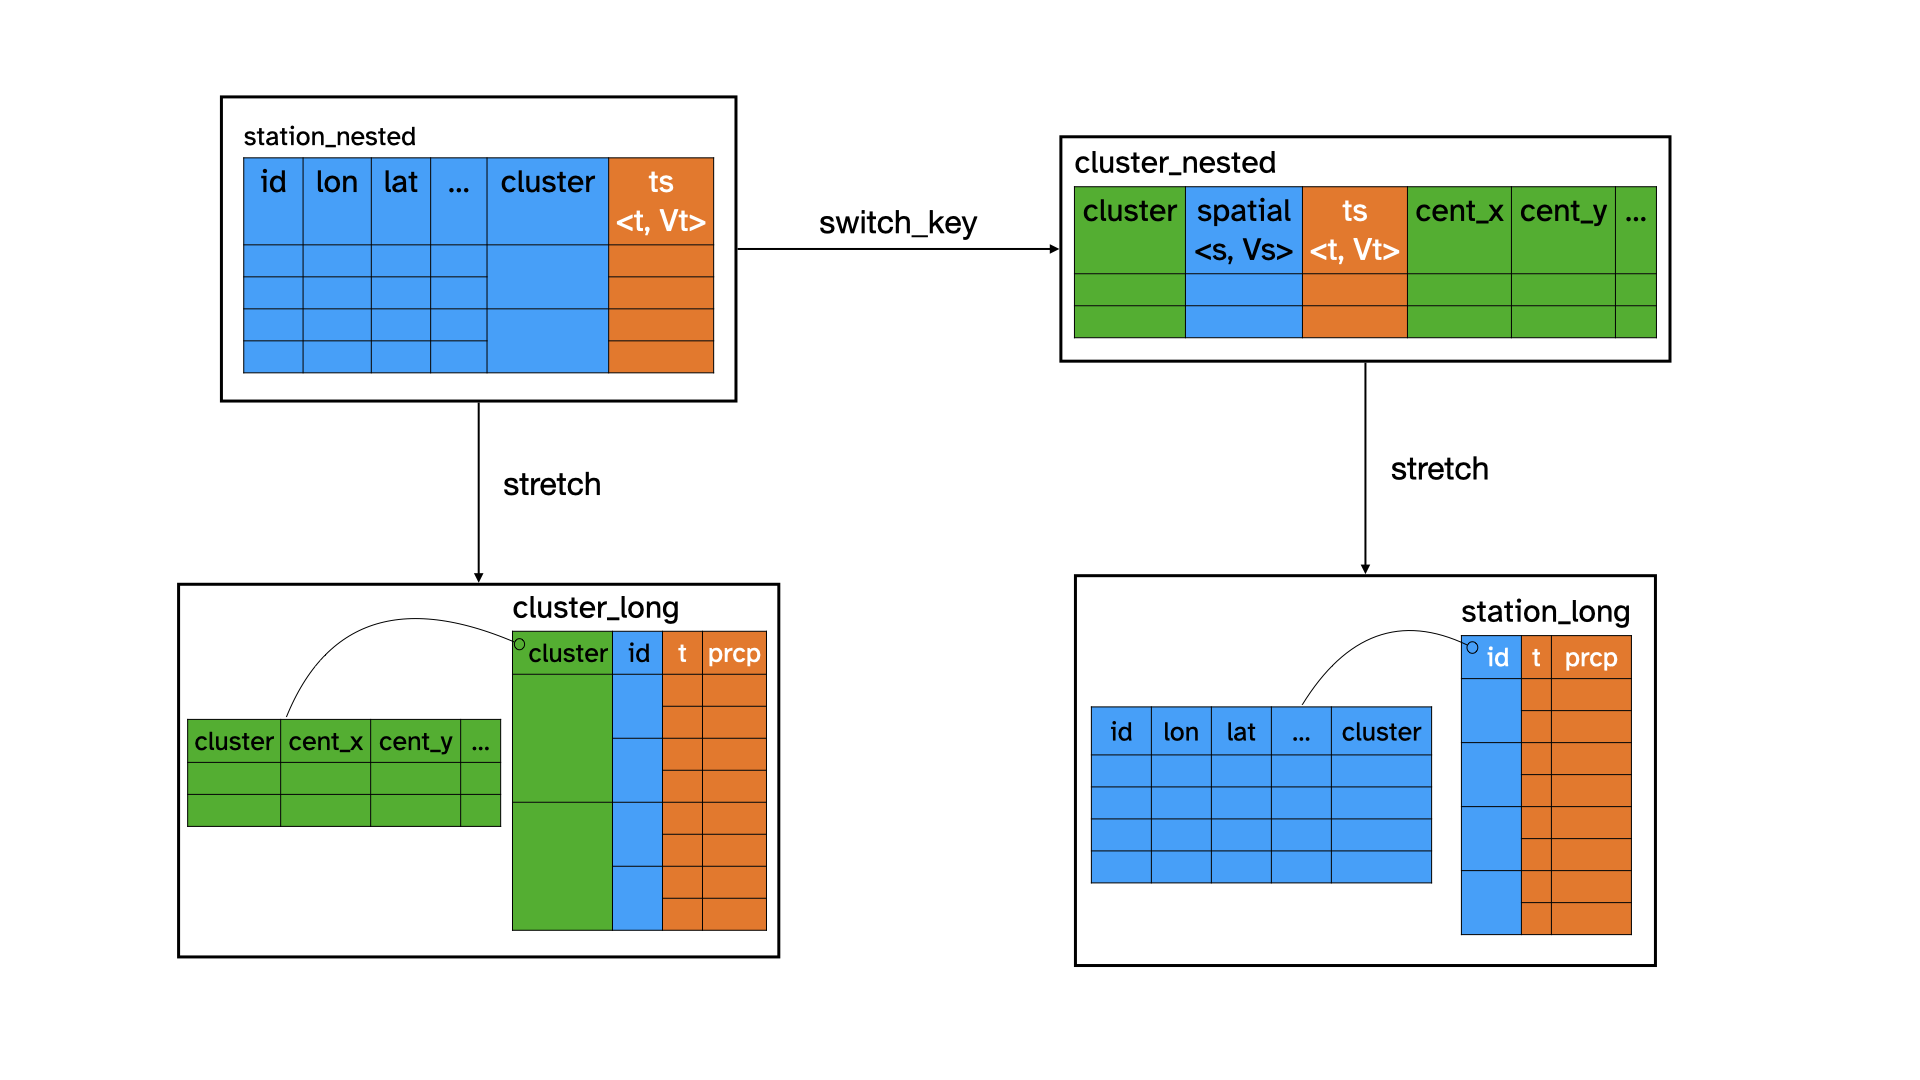
\includegraphics[width=1\linewidth,height=0.4\textheight]{/Users/sherryzhang/Documents/research/paper-cubble/figures/diagram-keynotes/diagram-keynotes.003} 

}

\caption{An illustration of the original and cluster level cubble in the nested form long form for hierarchical structure data. \code{switch\_key()} changes the station level cubble into a cluster level cubble and both can be stretched into the long form.}\label{fig:illu-hier}
\end{figure}

\hypertarget{data-fusion-and-matching}{%
\subsection{Data fusion and matching}\label{data-fusion-and-matching}}

One task that may interest analysts in spatio-temporal data is to find
how similar the time series from nearby sites are. This can be seen as a
matching problem (\protect\hyperlink{ref-stuart2010matching}{Stuart
2010}; \protect\hyperlink{ref-mcintosh2018using}{McIntosh et al. 2018})
that pairs up similar similar time series in nearby locations or a data
fusing exercise that merges data collected from different sources
(\protect\hyperlink{ref-cocchi2019data}{Cocchi 2019}).
\code{match_sites()} in \pkg{cubble} provides a simple algorithm for
this task. The algorithm first matches the two data sources spatially
through computing the pairwise distance on latitude and longitude. Pairs
that pass the spatial matching are then matched temporally through
computing the number of matched peaks within a fixed length window.
Figure \ref{fig:illu-matching} illustrates this temporal matching in
more details. Given two series \code{A} and \code{a}, 3 peaks have been
picked in each series. An interval, with default length of 5, is
constructed for each peak in series \code{A} and the peaks in series
\code{a} are tested against whether they fall into the any of the
intervals. In this illustration, there are 2 matches for these two
series. Several arguments are available in \code{match_sites()} to
fine-tune the matching:

\begin{figure}
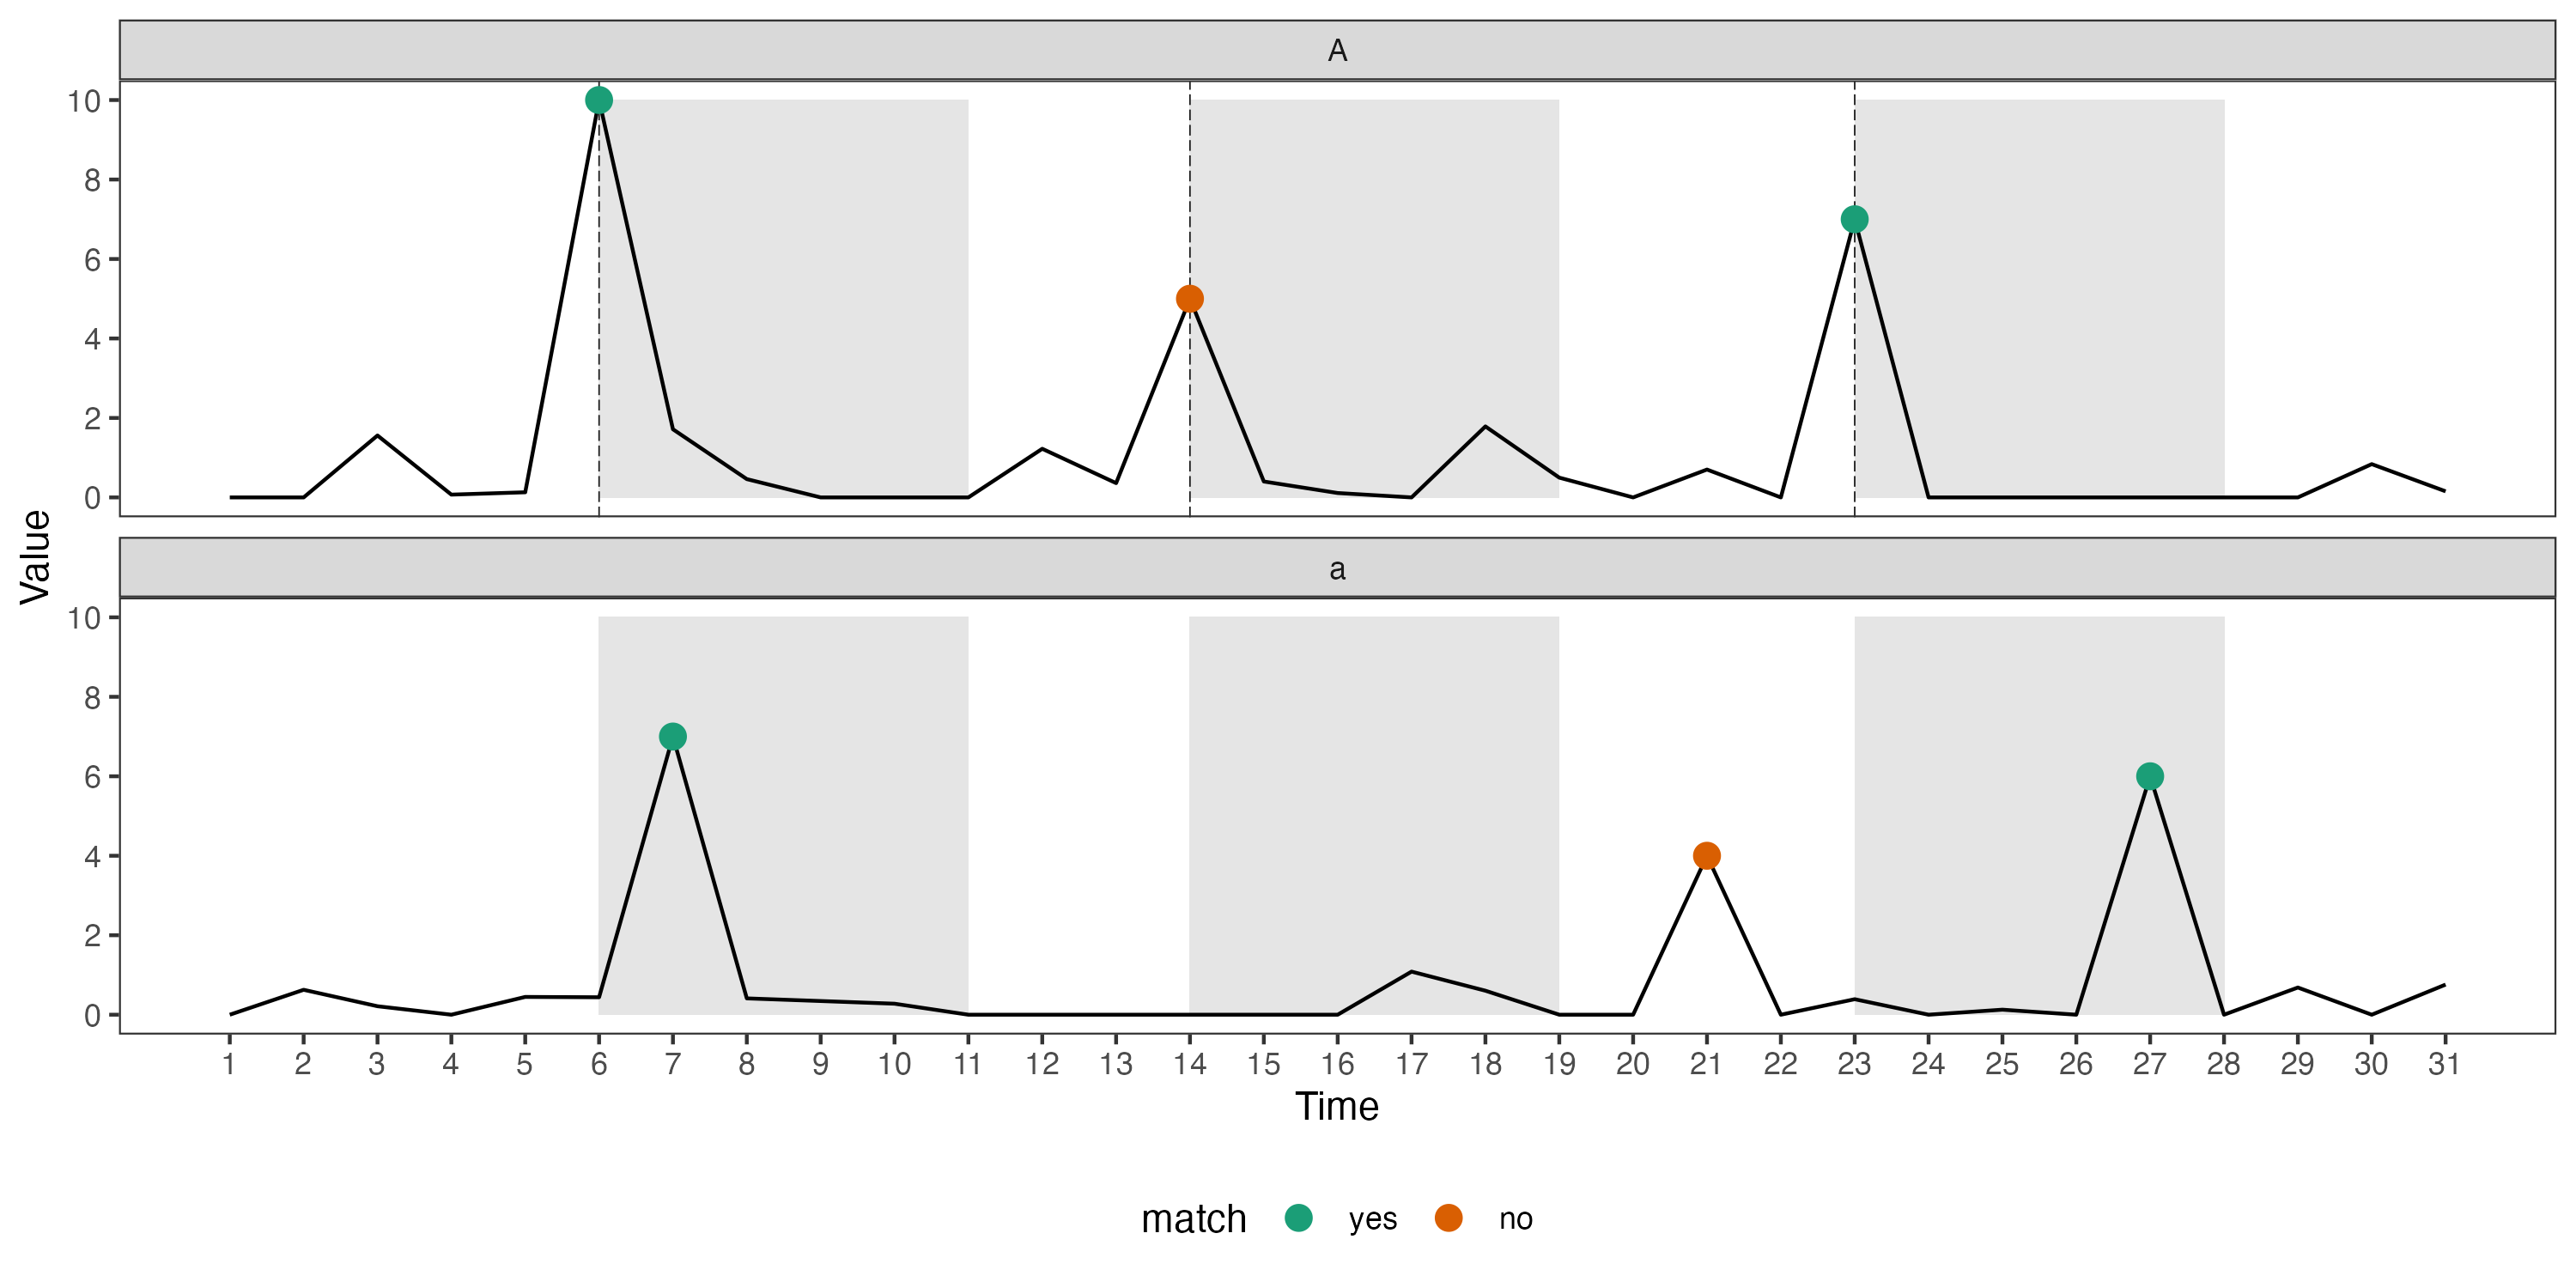
\includegraphics[width=1\linewidth]{/Users/sherryzhang/Documents/research/paper-cubble/figures/illu-matching} \caption{An illustration of temporal matching in cubble. Three highest peaks are identified in each series and intervals are constructed on series \code{A}. Two peaks in series \code{a} fall into the intervals and hence the two series are considered to have 2 matches.}\label{fig:illu-matching}
\end{figure}

\begin{itemize}
\tightlist
\item
  \code{spatial_n_keep}: the number of spatial match for each site to
  keep
\item
  \code{spatial_dist_max}: the maximum distance allowed for a matched
  pair
\item
  \code{temporal_n_highest}: the number of peak used - 3 in the example
  above
\item
  \code{temporal_window}: the length of the interval - 5 in the example
  above
\item
  \code{temporal_min_match}: the minimum number of matched peak for a
  valid matched pair
\end{itemize}

\hypertarget{interactive-graphics}{%
\subsection{Interactive graphics}\label{interactive-graphics}}

Cubble fits in naturally with the interactive graphic pipeline discussed
in the literature (\protect\hyperlink{ref-buja1988elements}{Buja,
Asimov, and Hurley 1988};
\protect\hyperlink{ref-buja1996interactive}{Buja, Cook, and Swayne
1996}; \protect\hyperlink{ref-sutherland2000orca}{Sutherland et al.
2000}; \protect\hyperlink{ref-xie2014reactive}{Xie, Hofmann, and Cheng
2014}; \protect\hyperlink{ref-cheng2016enabling}{Cheng, Cook, and
Hofmann 2016}). Diagram \ref{fig:illu-interactive} illustrates how
linking works from the map to the time series in cubble. The map and
time series plot is associated with the nested or long cubble,
respectively, and when a user action is captured on the map, the site
will be activated in the nested cubble (left). The nested cubble will
communicate to the long cubble to activate all the observations with the
same \code{id} (middle). The long cubble will then highlight the
activated series in the time series plot (right).

The linking is also available from the time series plot to the map. The
selection(s) on the time series is through selecting the point(s) on the
time series and once a point is selected, it will be activated in the
long cubble. All the observations that share the same \code{id} are then
activated and this includes other points in the same time series in the
long cubble and the corresponding observation of site in the nested
cubble. These activated observations will then being reflected in the
updated plots and Diagram \ref{fig:illu-interactive-2} in the Appendix
illustrates this process.

\begin{figure}

{\centering 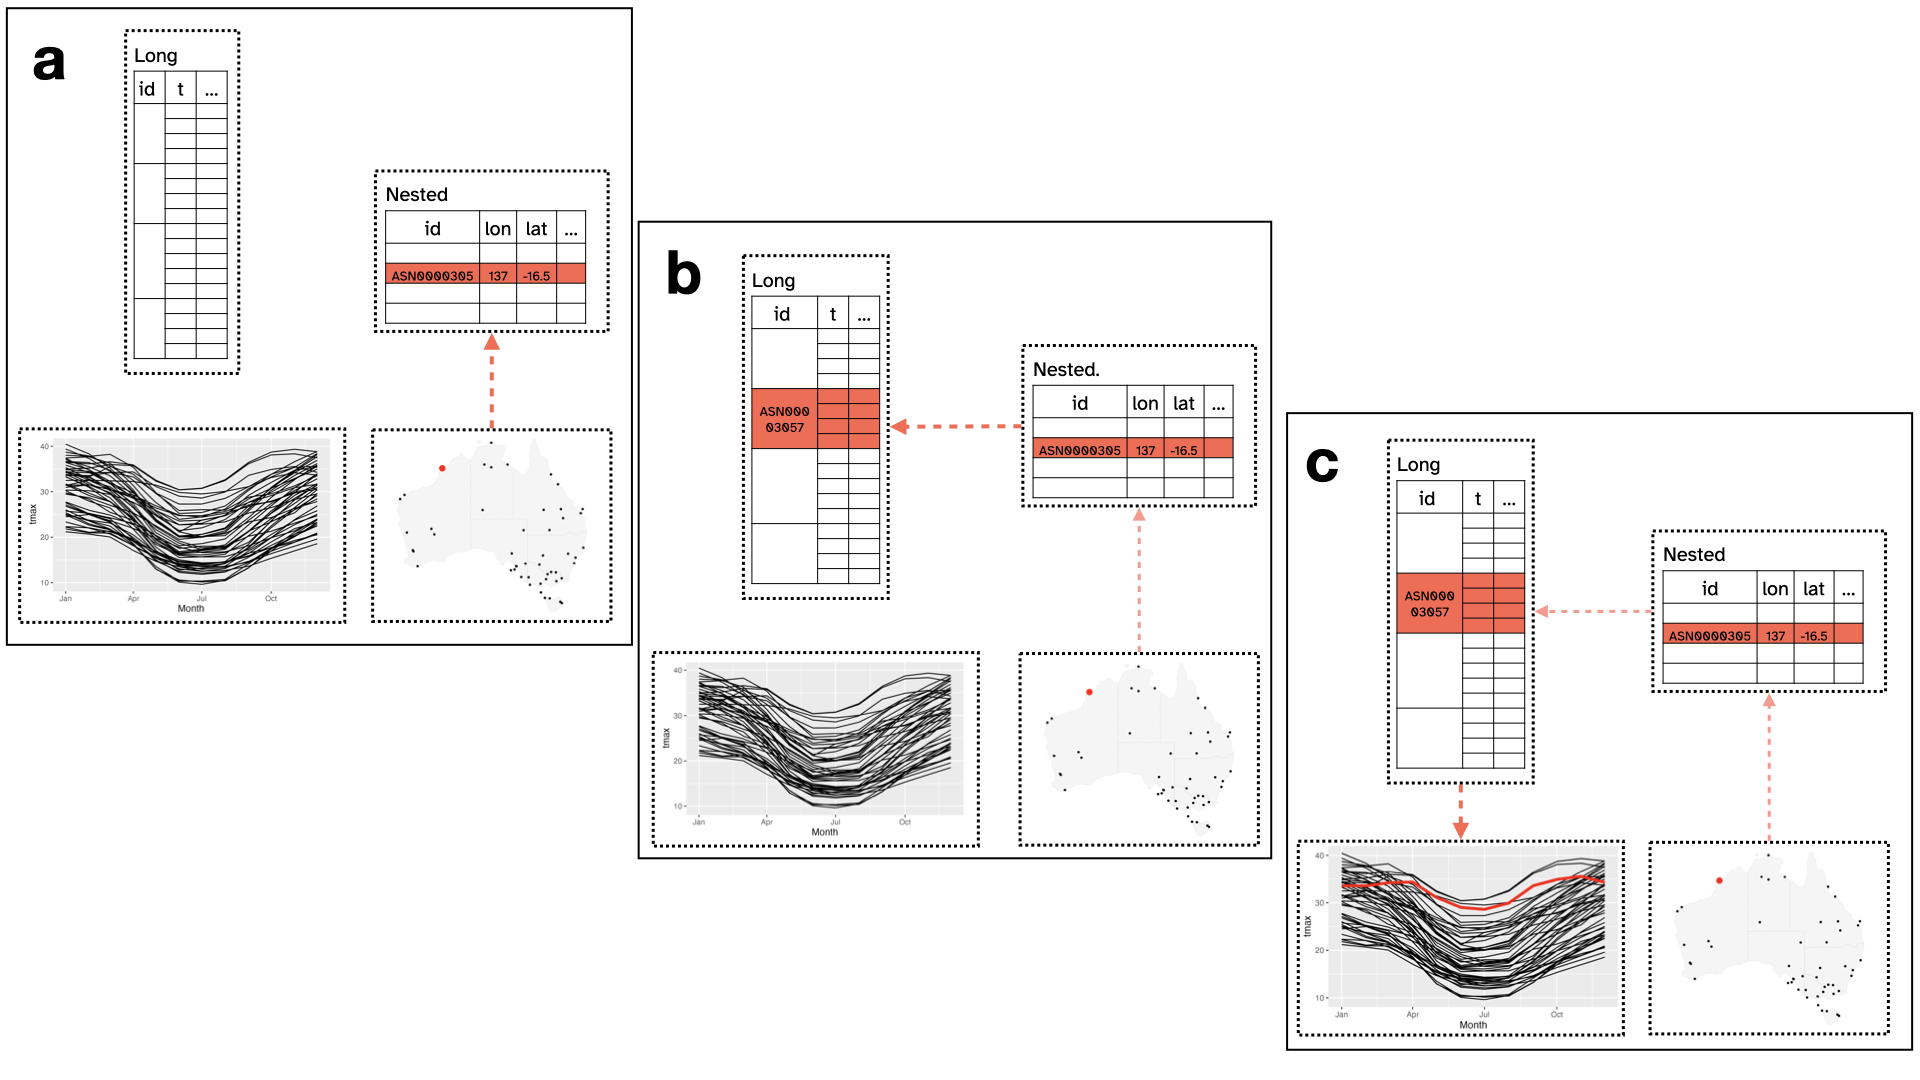
\includegraphics[width=1\linewidth,height=0.4\textheight]{/Users/sherryzhang/Documents/research/paper-cubble/figures/diagram-keynotes/diagram-keynotes.004} 

}

\caption{An illustration of the data model under interactive graphics with cubble. The line plot and the map is made separately with the long and nested cubble. When a station is selected on the map (left), the corresponding row in the nested cubble will be activated. This will link to all the rows with the same id in the long cubble (middle) and update the line plot (right).}\label{fig:illu-interactive}
\end{figure}

\hypertarget{st_transformation}{%
\subsection{Spatio-temporal transformations}\label{st_transformation}}

Spatio-temporal transformation is a useful technique to extract
information form spatio-temporal data. Glyph maps
(\protect\hyperlink{ref-Wickham2012-yr}{Wickham et al. 2012}) transform
the time coordinates into the space coordinates to plot the time series
of different locations on the map. Calendar plots
(\protect\hyperlink{ref-wang2020calendar}{Wang, Cook, and Hyndman
2020b}) reconstructs time into calendar-based grid to discover weekday
and weekend pattern. Projection, or linear combination, of variables
summarises multivariate information into lower dimension to further
digest. This section elaborates on the glyph map.

In \proglang{R}, \pkg{GGally} implements glyph maps through the
\code{glyphs()} function. The function constructs a data frame with
calculated position (\code{gx}. \code{gy}. \code{gid}) of each point on
the time series using linear algebra (Equation 1 and 2 in Wickham et al.
(\protect\hyperlink{ref-Wickham2012-yr}{2012})). The data can then be
piped into \code{ggplot} to create the glyph map as:

\begin{Shaded}
\begin{Highlighting}[]
\FunctionTok{library}\NormalTok{(ggplot2)}
\NormalTok{gly }\OtherTok{\textless{}{-}} \FunctionTok{glyphs}\NormalTok{(data, }
              \AttributeTok{x\_major =}\NormalTok{ ..., }\AttributeTok{x\_minor =}\NormalTok{ ..., }
              \AttributeTok{y\_major =}\NormalTok{ ..., }\AttributeTok{y\_minor =}\NormalTok{ ..., ...)}

\FunctionTok{ggplot}\NormalTok{(gly, }\FunctionTok{aes}\NormalTok{(gx, gy, }\AttributeTok{group =}\NormalTok{ gid)) }\SpecialCharTok{+} 
  \FunctionTok{geom\_path}\NormalTok{() }
\end{Highlighting}
\end{Shaded}

A re-implementation of the glyph map as a ggproto, \code{GeomGlyph}, has
been made in the \pkg{cubble} package and now the glyph map can be
created with \code{geom_glyph()}:

\begin{Shaded}
\begin{Highlighting}[]
\FunctionTok{ggplot}\NormalTok{(}\AttributeTok{data =}\NormalTok{ data) }\SpecialCharTok{+}
  \FunctionTok{geom\_glyph}\NormalTok{(}\FunctionTok{aes}\NormalTok{(}\AttributeTok{x\_major =}\NormalTok{ ..., }\AttributeTok{x\_minor =}\NormalTok{ ..., }
                 \AttributeTok{y\_major =}\NormalTok{ ..., }\AttributeTok{y\_minor =}\NormalTok{ ...))}
\end{Highlighting}
\end{Shaded}

Some useful controls over the glyph map is also available in the
\code{geom_glyph()} implementation. Polar glyph map can be specify as a
parameter, \code{polar = TRUE}. in the \code{geom_glyph()}, along with
\code{width} and \code{height} in either absolute or relative value.
Global and local scale can be controlled by the parameter
\code{global_rescale}. which default to \code{TRUE} for global scaling.
Reference box and line can be added with separate
\code{geom_glyph_box()} and \code{geom_glyph_line()}.

\hypertarget{examples}{%
\section{Examples}\label{examples}}

\hypertarget{australia-historical-maximum-temperature}{%
\subsection{Australia historical maximum
temperature}\label{australia-historical-maximum-temperature}}

Global Historical Climatology Network (GHCN) provides daily climate
measures from stations across the world. The dataset
\code{weatherdata::historical_tmax} extracts the maximum temperature for
236 Australian stations from GHCN with starting from year 1969.
\code{weatherdata::historical_tmax} is already in a cubble, with
\code{id} as the key, \code{date} as the index, and
\code{c(longitude, latitude)} as the coordinates. This example compares
the maximum temperature in two periods: 1971 - 1975 and 2016 - 2020 for
stations in Victoria and New South Wales.

Stations in the two states can be subsetted by the station number:
Australia GHCN station number starts with ``ASN00'' and followed by the
\href{http://www.bom.gov.au/climate/cdo/about/site-num.shtml}{Bureau of
Meteorology (BOM) station number}, where the 2nd and 3rd digit (7th and
8th in the GHCN number) define the state of the station. New South Wales
stations start from 46 to 75 and Victoria stations follow from 76 to 90.
Filtering Victoria and New South Wales stations is an operation in the
spatial dimension and hence uses the nested form:

\begin{Shaded}
\begin{Highlighting}[]
\NormalTok{tmax }\OtherTok{\textless{}{-}}\NormalTok{ weatherdata}\SpecialCharTok{::}\NormalTok{historical\_tmax }\SpecialCharTok{|}\ErrorTok{\textgreater{}}
  \FunctionTok{filter}\NormalTok{(}\FunctionTok{between}\NormalTok{(stringr}\SpecialCharTok{::}\FunctionTok{str\_sub}\NormalTok{(id, }\DecValTok{7}\NormalTok{, }\DecValTok{8}\NormalTok{), }\DecValTok{46}\NormalTok{, }\DecValTok{90}\NormalTok{))}
\end{Highlighting}
\end{Shaded}

Filtering for the period 1971 \textasciitilde{} 1975 and 2016
\textasciitilde{} 2020 is an operation on the time dimension and the
nested cubble needs to be switched to the long cubble by
\code{stretch()}:

\begin{Shaded}
\begin{Highlighting}[]
\NormalTok{tmax }\OtherTok{\textless{}{-}}\NormalTok{ tmax }\SpecialCharTok{|}\ErrorTok{\textgreater{}} 
  \FunctionTok{face\_temporal}\NormalTok{() }\SpecialCharTok{|}\ErrorTok{\textgreater{}}
  \FunctionTok{filter}\NormalTok{(lubridate}\SpecialCharTok{::}\FunctionTok{year}\NormalTok{(date) }\SpecialCharTok{\%in\%} \FunctionTok{c}\NormalTok{(}\DecValTok{1971}\SpecialCharTok{:}\DecValTok{1975}\NormalTok{, }\DecValTok{2016}\SpecialCharTok{:}\DecValTok{2020}\NormalTok{)) }
\end{Highlighting}
\end{Shaded}

A monthly average is used for both periods to smooth the maximum
temperature and it is again an operation on the time dimension:

\begin{Shaded}
\begin{Highlighting}[]
\NormalTok{tmax }\OtherTok{\textless{}{-}}\NormalTok{ tmax }\SpecialCharTok{|}\ErrorTok{\textgreater{}}
  \FunctionTok{group\_by}\NormalTok{(}\AttributeTok{month =}\NormalTok{ lubridate}\SpecialCharTok{::}\FunctionTok{month}\NormalTok{(date), }
         \AttributeTok{group =} \FunctionTok{as.factor}\NormalTok{(}\FunctionTok{ifelse}\NormalTok{(lubridate}\SpecialCharTok{::}\FunctionTok{year}\NormalTok{(date) }\SpecialCharTok{\textgreater{}} \DecValTok{2015}\NormalTok{, }
                                  \StringTok{"2016 \textasciitilde{} 2020"}\NormalTok{, }\StringTok{"1971 \textasciitilde{} 1975"}\NormalTok{))) }\SpecialCharTok{|}\ErrorTok{\textgreater{}}
  \FunctionTok{summarise}\NormalTok{(}\AttributeTok{tmax =} \FunctionTok{mean}\NormalTok{(tmax, }\AttributeTok{na.rm =} \ConstantTok{TRUE}\NormalTok{))}
\end{Highlighting}
\end{Shaded}

A few stations don't have records during 1971 - 1975 and further
investigation shows that while the first and last year of each series is
recorded, the missing years in this period is not reported. These
stations are filtered out by examining whether the summarised time
series has a total of 24 months. The long cubble needs to be switched to
the nested form for this spatial operation using \code{face_spatial()}:

\begin{Shaded}
\begin{Highlighting}[]
\NormalTok{tmax }\OtherTok{\textless{}{-}}\NormalTok{ tmax }\SpecialCharTok{|}\ErrorTok{\textgreater{}} \FunctionTok{face\_spatial}\NormalTok{() }\SpecialCharTok{|}\ErrorTok{\textgreater{}} \FunctionTok{filter}\NormalTok{(}\FunctionTok{nrow}\NormalTok{(ts) }\SpecialCharTok{==} \DecValTok{24}\NormalTok{) }
\end{Highlighting}
\end{Shaded}

Lastly, to create a glyph map, both the major (\code{longitude},
\code{latitude}) and minor (\code{month}, \code{tmax}) coordinates need
to be in the same table. Spatial variables can be moved to the long form
with \code{migrate()}:

\begin{Shaded}
\begin{Highlighting}[]
\NormalTok{tmax }\OtherTok{\textless{}{-}}\NormalTok{ tmax }\SpecialCharTok{|}\ErrorTok{\textgreater{}} \FunctionTok{face\_temporal}\NormalTok{() }\SpecialCharTok{|}\ErrorTok{\textgreater{}} \FunctionTok{unfold}\NormalTok{(latitude, longitude)}
\end{Highlighting}
\end{Shaded}

\code{tmax} can then be supplied to \code{geom_glyph()} for the glyph
map in Figure \ref{fig:basic-manip} with a station inset on the top left
corner:

\begin{Shaded}
\begin{Highlighting}[]
\NormalTok{nsw\_vic }\OtherTok{\textless{}{-}}\NormalTok{ ozmaps}\SpecialCharTok{::}\NormalTok{abs\_ste }\SpecialCharTok{|}\ErrorTok{\textgreater{}} 
  \FunctionTok{filter}\NormalTok{(NAME }\SpecialCharTok{\%in\%} \FunctionTok{c}\NormalTok{(}\StringTok{"Victoria"}\NormalTok{, }\StringTok{"New South Wales"}\NormalTok{))}

\FunctionTok{ggplot}\NormalTok{() }\SpecialCharTok{+} 
  \FunctionTok{geom\_sf}\NormalTok{(}\AttributeTok{data =}\NormalTok{ nsw\_vic, }
          \AttributeTok{fill =} \StringTok{"transparent"}\NormalTok{, }\AttributeTok{color =} \StringTok{"grey"}\NormalTok{, }\AttributeTok{linetype =} \StringTok{"dotted"}\NormalTok{) }\SpecialCharTok{+} 
  \FunctionTok{geom\_glyph}\NormalTok{(}\AttributeTok{data =}\NormalTok{ tmax, }
             \FunctionTok{aes}\NormalTok{(}\AttributeTok{x\_major =}\NormalTok{ longitude, }\AttributeTok{x\_minor =}\NormalTok{ month, }
                 \AttributeTok{y\_major =}\NormalTok{ latitude, }\AttributeTok{y\_minor =}\NormalTok{ tmax,}
                 \AttributeTok{group =} \FunctionTok{interaction}\NormalTok{(id, group), }\AttributeTok{color =}\NormalTok{ group),}
             \AttributeTok{width =} \DecValTok{1}\NormalTok{, }\AttributeTok{height =} \FloatTok{0.5}\NormalTok{) }\SpecialCharTok{+}
\NormalTok{  ...}
\end{Highlighting}
\end{Shaded}

\begin{figure}
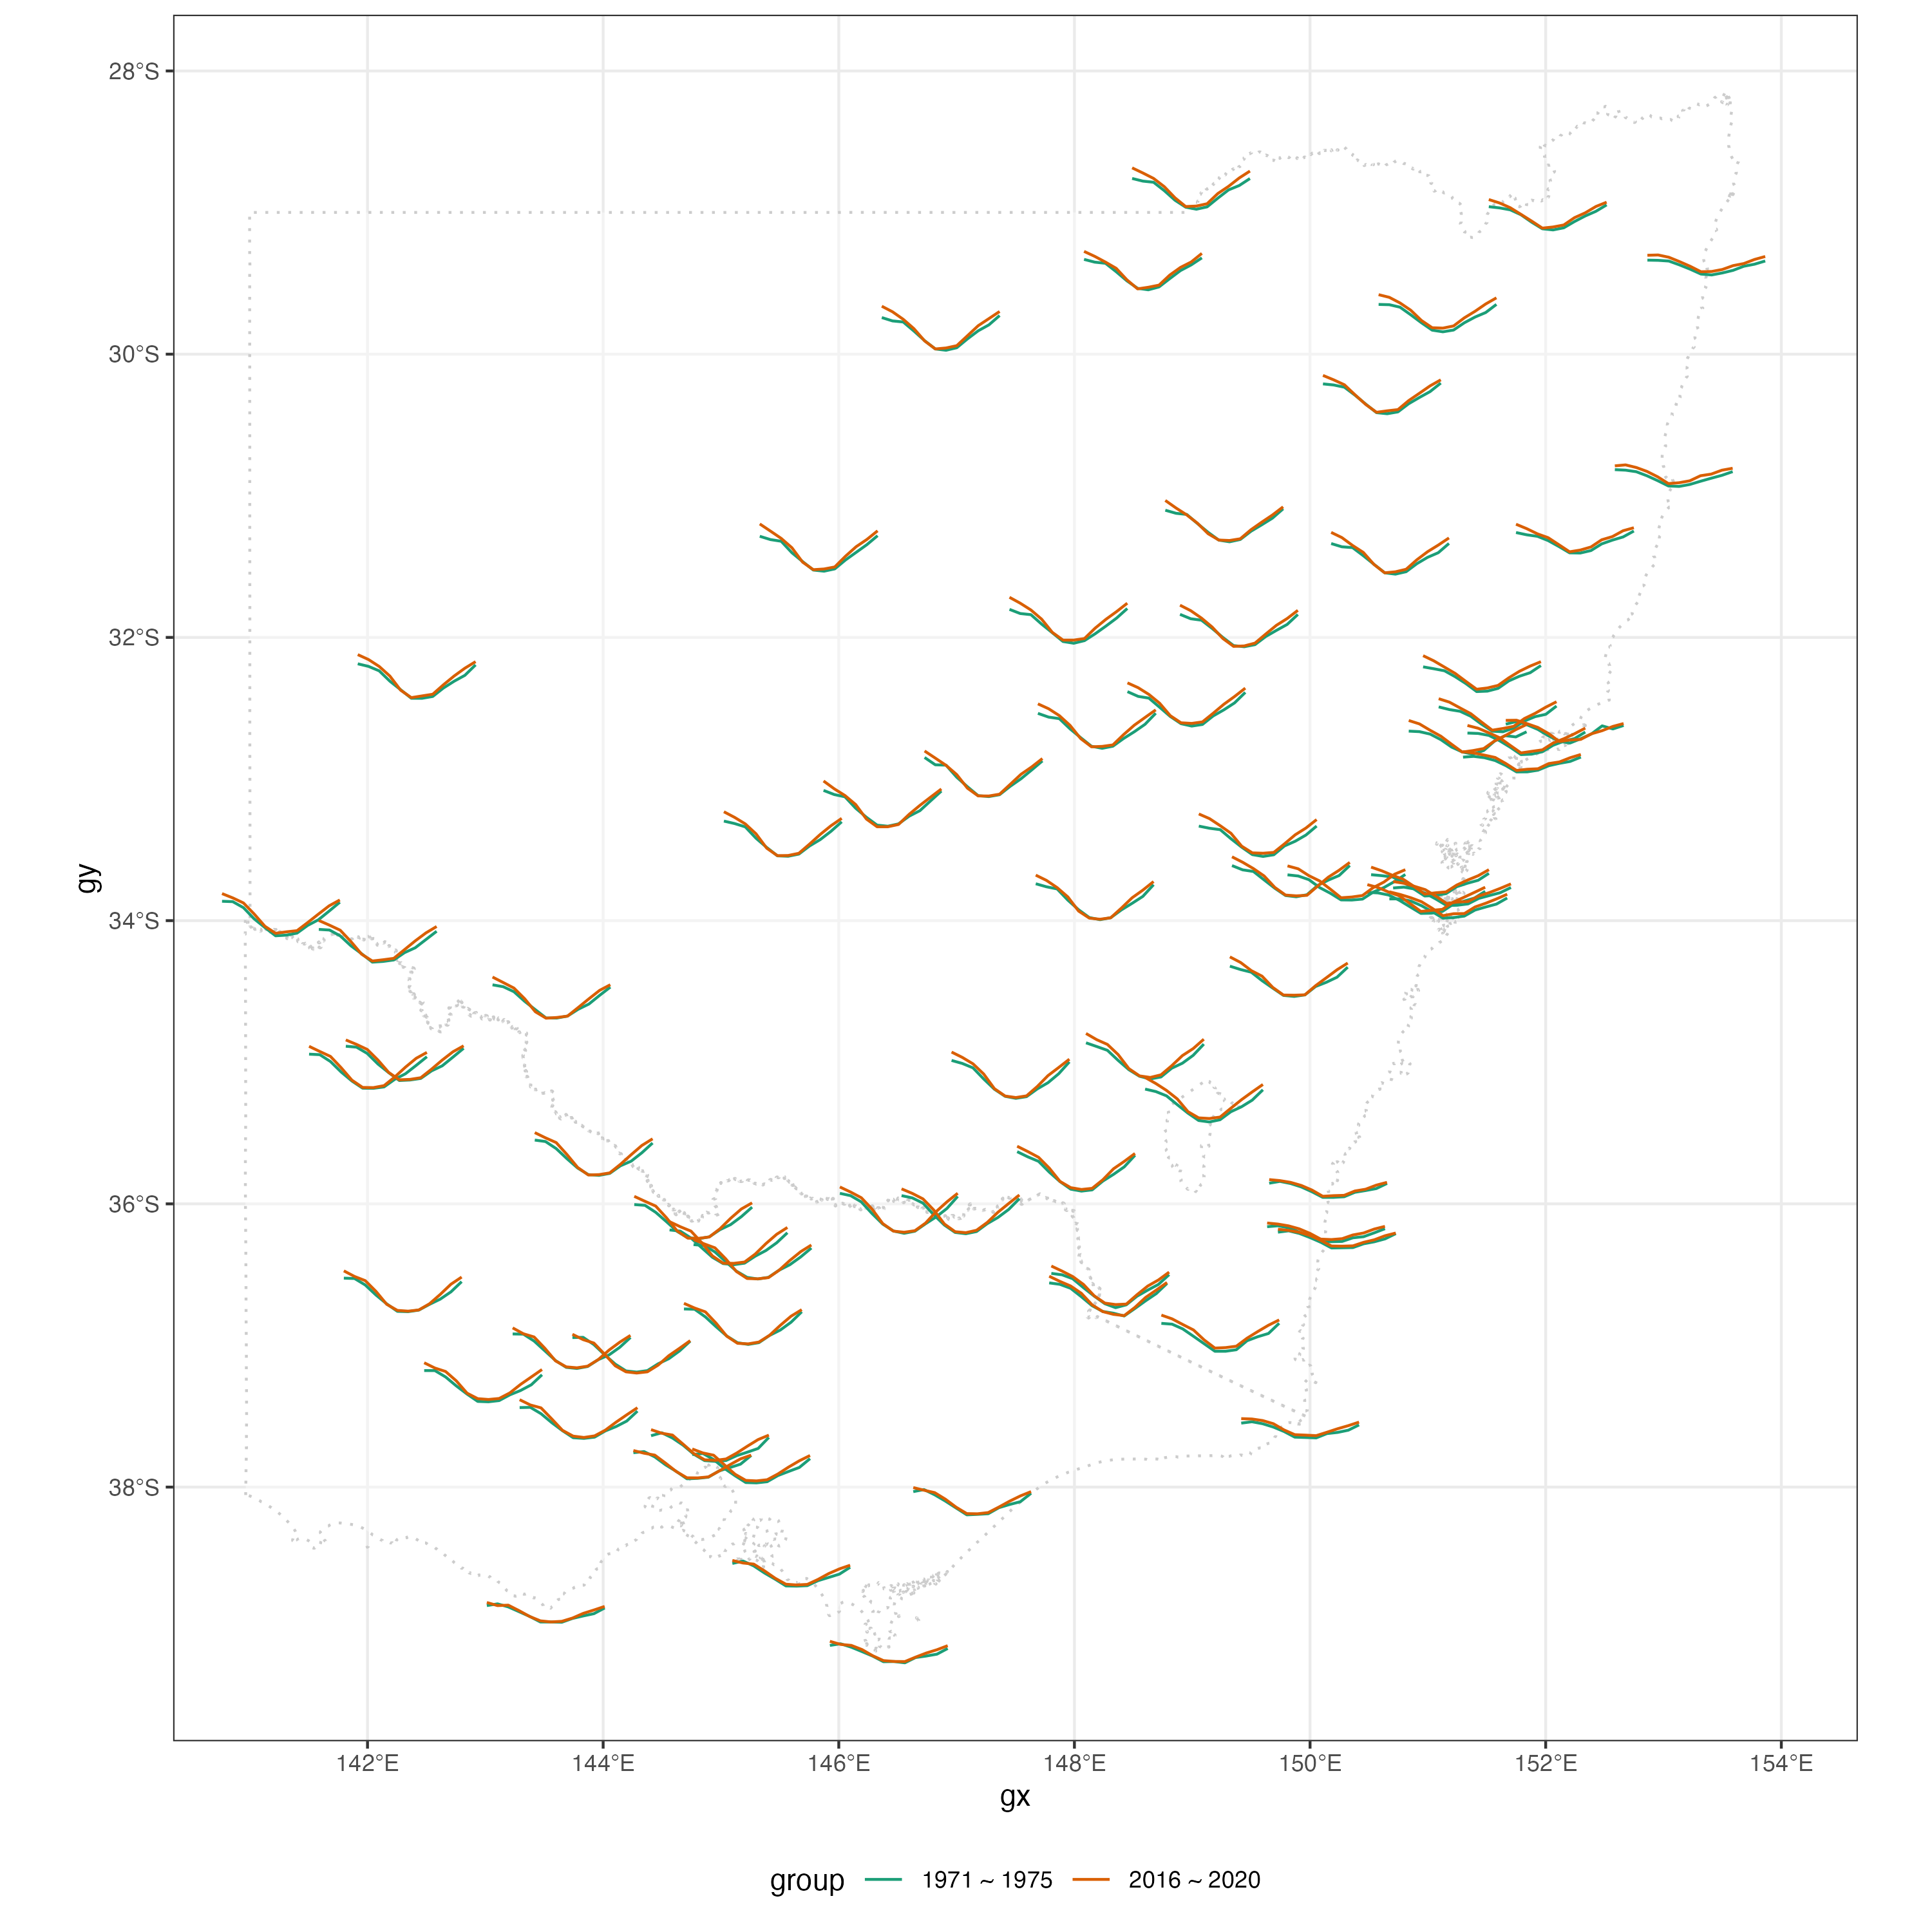
\includegraphics[width=1\linewidth,height=0.7\textheight]{/Users/sherryzhang/Documents/research/paper-cubble/figures/basic-manip} \caption{A glyph map of the average maximum temperature by month of Victoria and New South Wales weather stations in Australia. On the top left corner is an insetted plot of station Cobar highlighted in the black box.}\label{fig:basic-manip}
\end{figure}

\hypertarget{australia-precipitation-pattern-in-2020}{%
\subsection{Australia precipitation pattern in
2020}\label{australia-precipitation-pattern-in-2020}}

In the previous example, there has already been some overlapping of the
glyphs for a few stations near (151E, 34S) and (152E, 33S) and this will
be a problem when mapping more stations in the national level.
Aggregation can be helpful to group series into clusters before
visualising the cluster with glyph map. This example shows how to
organise data at both level with \code{switch_key()}.

\code{weatherdata::climate_full}, also extracted from GHCN, records
daily precipitation and maximum/ minimum temperature for 639 stations in
Australia from 2016 to 2020. A simple kmean algorithm based on the
distance matrix is used to create 20 clusters. This creates
\code{station_nested} as a station level nested cubble with a cluster
column indicating the group each station belongs to. More complex
algorithms can be used for other problem, as long as there is a mapping
from each station to a cluster.

\begin{Shaded}
\begin{Highlighting}[]
\NormalTok{station\_nested }\OtherTok{\textless{}{-}}\NormalTok{ weatherdata}\SpecialCharTok{::}\NormalTok{climate\_full }\SpecialCharTok{|}\ErrorTok{\textgreater{}} 
  \FunctionTok{mutate}\NormalTok{(}\AttributeTok{cluster =}\NormalTok{ ...)}
\end{Highlighting}
\end{Shaded}

To create a group level cubble, use \code{switch_key()} with the new key
variable, \code{cluster}:

\begin{Shaded}
\begin{Highlighting}[]
\NormalTok{cluster\_nested }\OtherTok{\textless{}{-}}\NormalTok{ station\_nested }\SpecialCharTok{|}\ErrorTok{\textgreater{}} \FunctionTok{switch\_key}\NormalTok{(cluster) }
\end{Highlighting}
\end{Shaded}

With the group level cubble, \code{get_centroid()} is useful to compute
the centroid of each cluster, which will be used as the major axis for
the glyph map later:

\begin{Shaded}
\begin{Highlighting}[]
\NormalTok{cluster\_nested }\OtherTok{\textless{}{-}}\NormalTok{ cluster\_nested }\SpecialCharTok{|}\ErrorTok{\textgreater{}} \FunctionTok{get\_centroid}\NormalTok{()}
\end{Highlighting}
\end{Shaded}

Long form cubble at both levels can be accessed through stretching the
nested form and with access to both station and cluster level cubbles,
various plots can be made to understand the cluster. Figure
\ref{fig:basic-agg} shows two example plots that can be made with this
data: subplot A is a glyph map made with the cluster level cubble in the
long form and subplot B inspects the station membership of each cluster
using the station level cubble in the nested form.

\begin{figure}
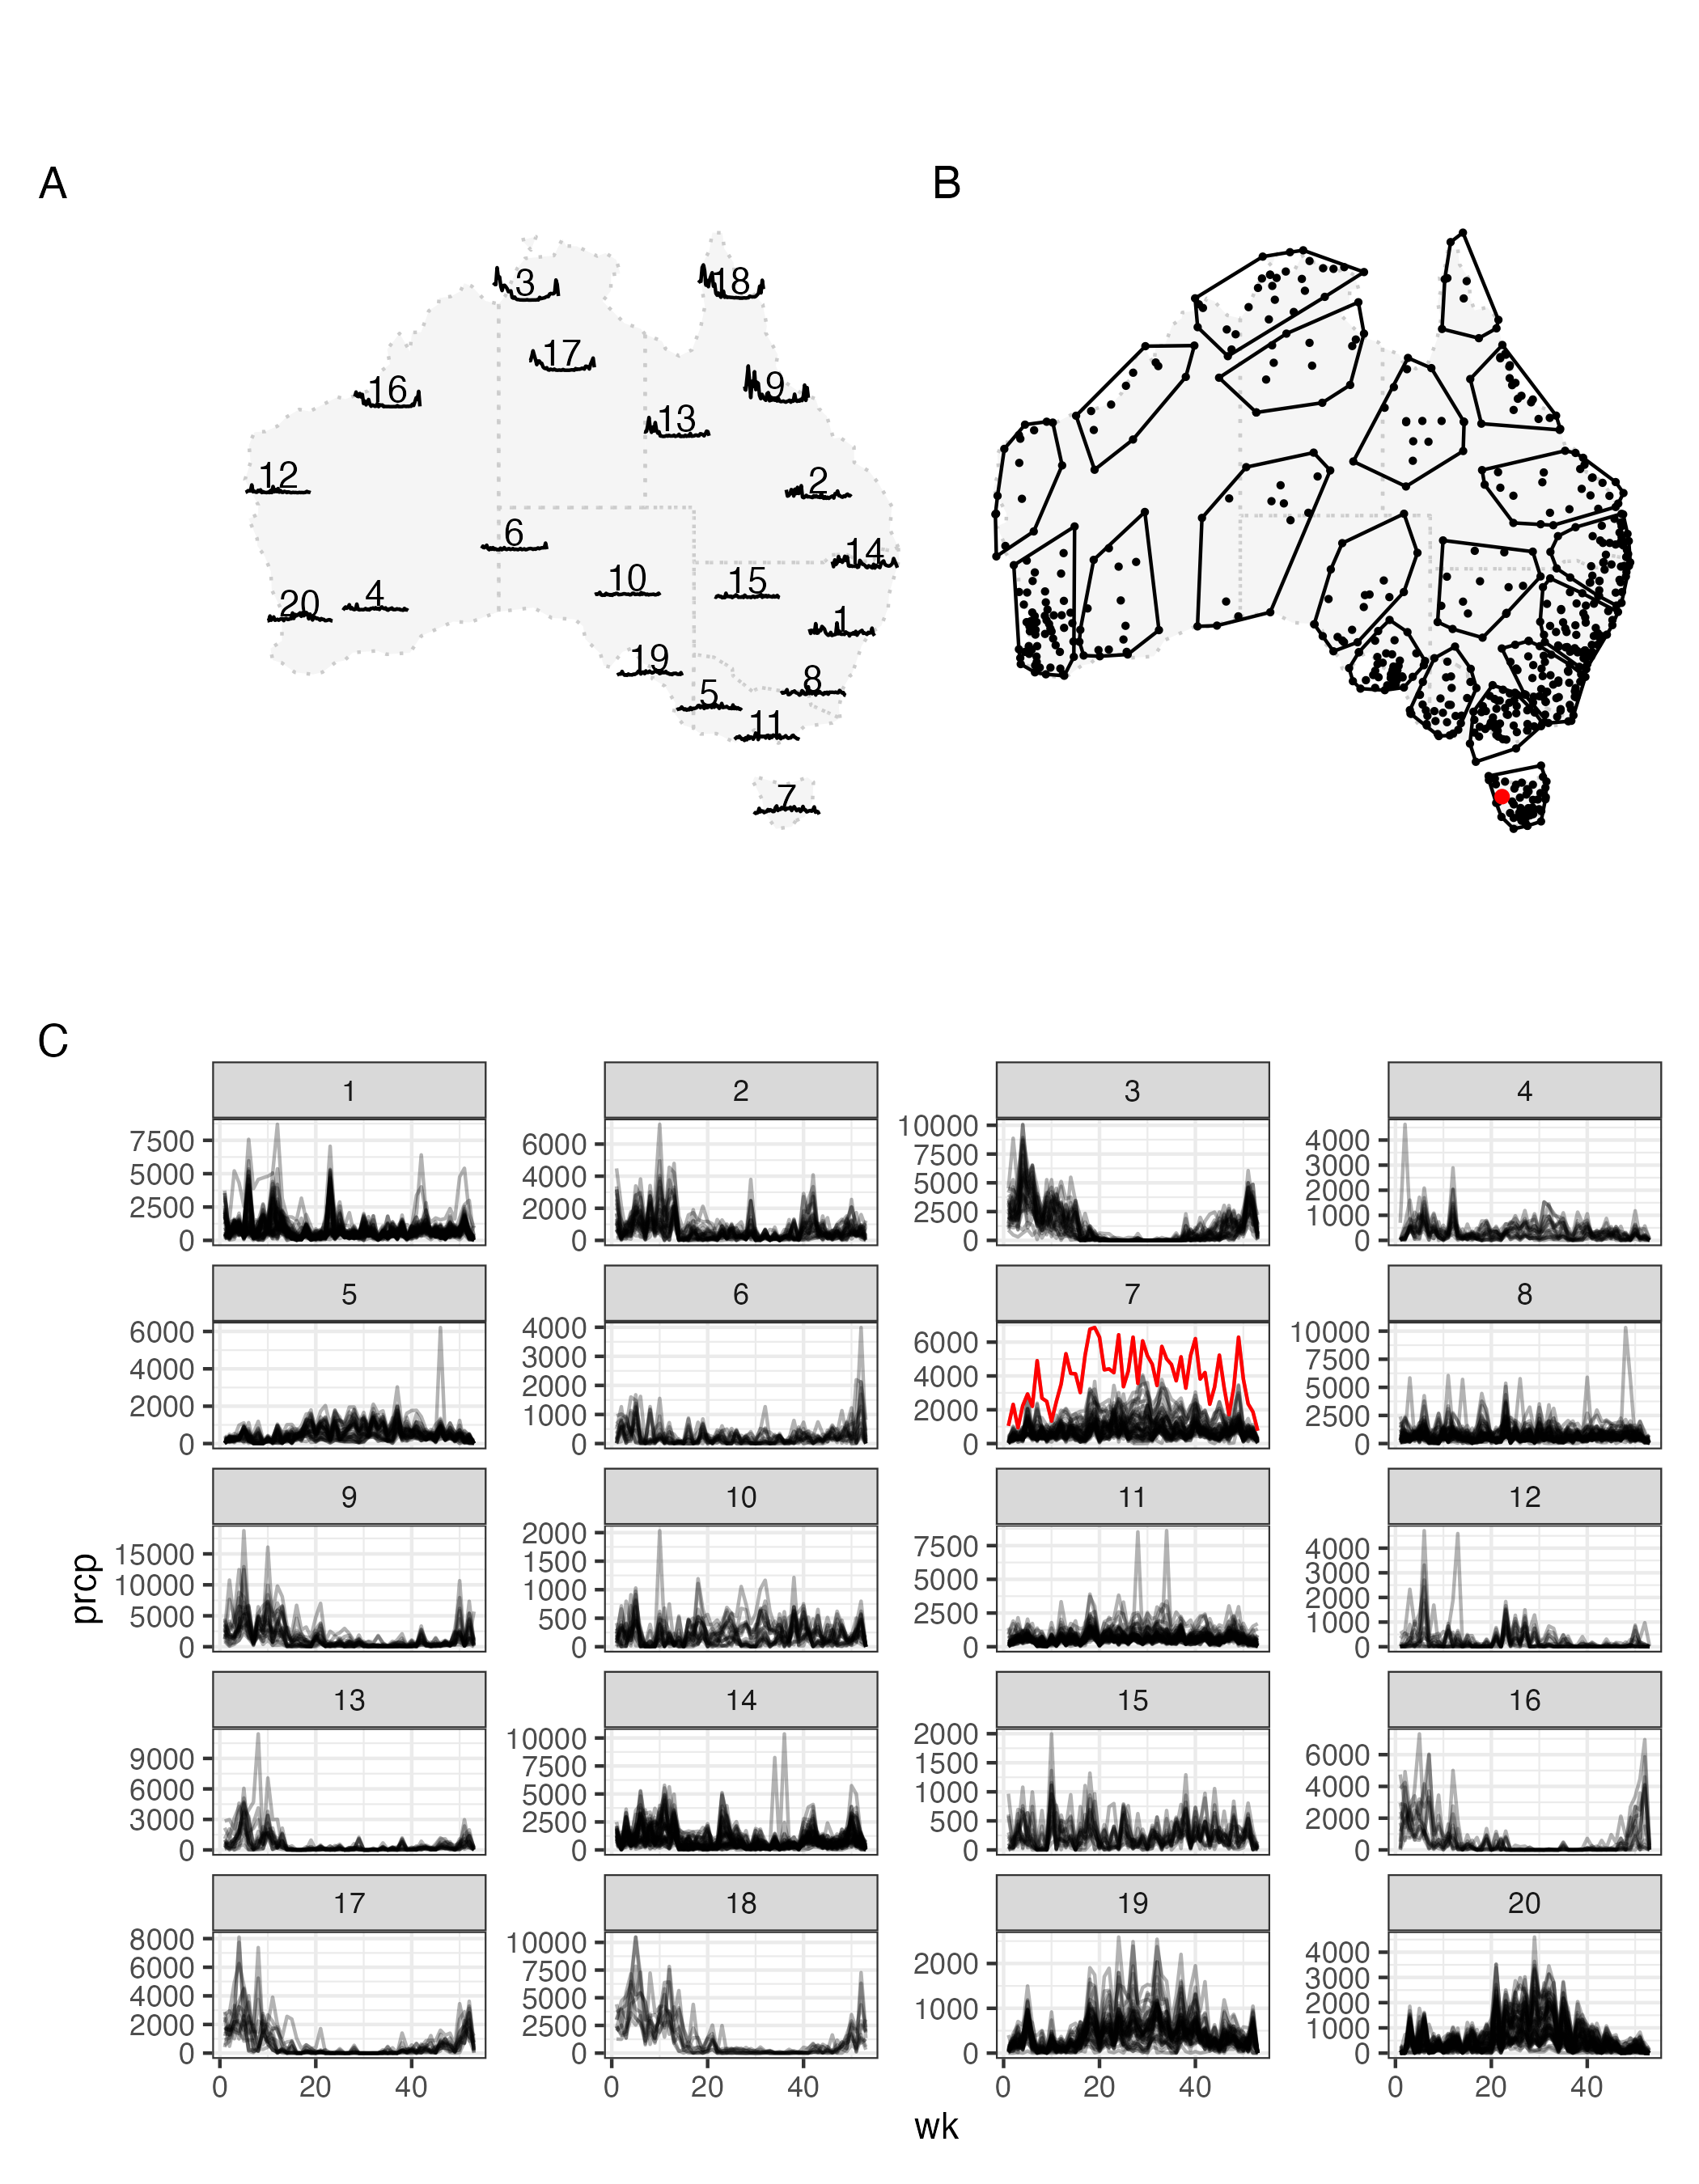
\includegraphics[width=1\linewidth]{/Users/sherryzhang/Documents/research/paper-cubble/figures/basic-agg} \caption{Profile of aggregated precipitation from 639 weather stations in Australia. Subplot A shows the glyph map of the weekly averaged precipitation of each cluster. The group number of printed in the middle of y minor axis and can be used as a reference line to read the magnitude. Subplot B shows the station membership of each cluster.}\label{fig:basic-agg}
\end{figure}

\hypertarget{river-level-data-in-victoria-water-gauges}{%
\subsection{River level data in Victoria water
gauges}\label{river-level-data-in-victoria-water-gauges}}

Bureau of Meteorology collects
\href{http://www.bom.gov.au/metadata/catalogue/19115/ANZCW0503900528?template=full}{water
data} from river gauges and this includes variables: electrical
conductivity, turbidity, water course discharge, water course level, and
water temperature. In particular, water level will interactive with
precipitation from the climate data since rainfall will raise the water
level in the river. Figure \ref{fig:matching-map} gives the location of
available weather station and water gauges in Victoria.

\begin{figure}
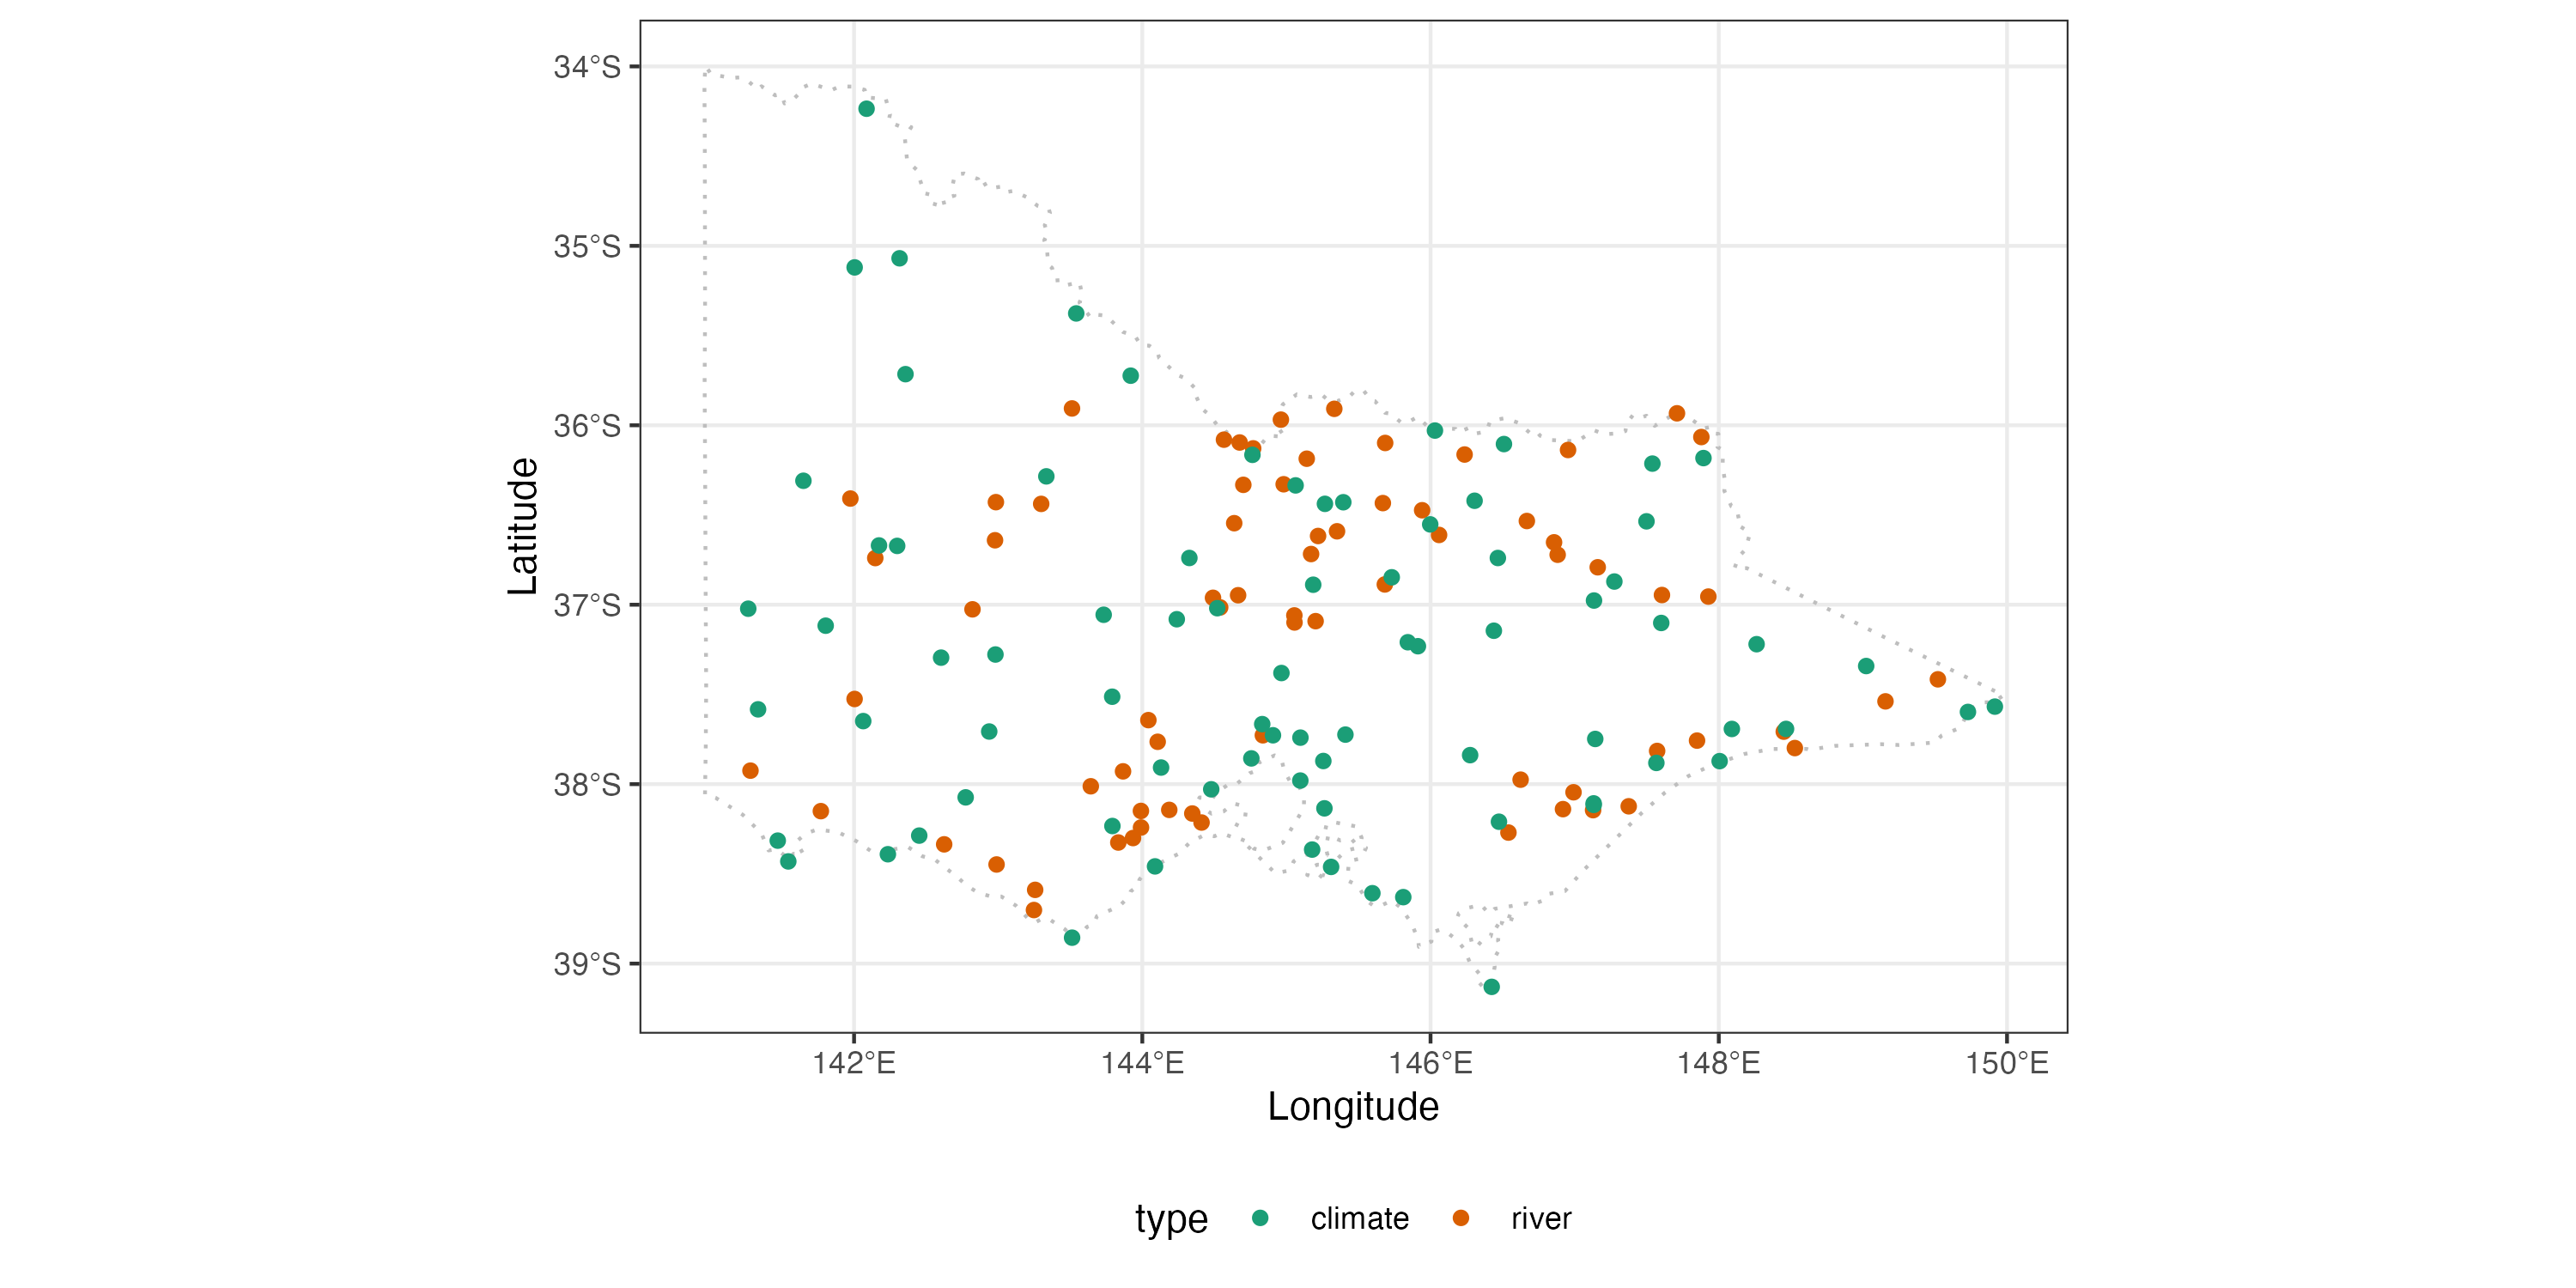
\includegraphics[width=1\linewidth]{/Users/sherryzhang/Documents/research/paper-cubble/figures/matching-map} \caption{Location of weather stations and river gauges in Victoria, Australia.}\label{fig:matching-map}
\end{figure}

From the map, a few water gauges and weather stations are close to each
other and the fluctuation of the water level could be matched up with
precipitation measured by the climate station. As introduced in Section
3.2, \code{match_sites()} can be used to match one source of data with
another source in a cubble. Here \code{Water_course_level} in
\code{river} will be matched to \code{prcp} in \code{climate} in 2020.
The two datasets need to be specified as the first two arguments and the
variable to match can be specified in \code{temporal_by} using the
\code{by} syntax in \code{join}. \code{temporal_independent} controls
the variable used to construct the interval and the goal here is to see
if precipitation will be reflected by the water level in the river. This
puts precipitation \code{prcp}, as the independent. Given there is one
year worth of data, the number of peak (\code{temporal_n_highest}) to
consider is slightly raised from a default 20 to 30 and
\code{temporal_min_match} is raised accordingly To return all the pairs
of the match, \code{temporal_min_match} can be set to 0.

\begin{Shaded}
\begin{Highlighting}[]
\NormalTok{res }\OtherTok{\textless{}{-}} \FunctionTok{match\_sites}\NormalTok{(}
\NormalTok{  river, climate,}
  \AttributeTok{temporal\_by =} \FunctionTok{c}\NormalTok{(}\StringTok{"Water\_course\_level"} \OtherTok{=} \StringTok{"prcp"}\NormalTok{),}
  \AttributeTok{temporal\_independent =} \StringTok{"prcp"}\NormalTok{,  }
  \AttributeTok{temporal\_n\_highest =} \DecValTok{30}\NormalTok{,}
  \AttributeTok{temporal\_min\_match =} \DecValTok{15}
\NormalTok{)}
\end{Highlighting}
\end{Shaded}

The output from matching is also a cubble, with additional column
\code{dist} and \code{group} produced from spatial matching and
\code{n_match} from temporal matching.

\begin{verbatim}
## # cubble:   id [8]: nested form
## # bbox:     [144.52, -37.73, 146.06, -36.55]
## # temporal: date [date], matched_var [dbl]
##   id          name                  lat  long type   dist group ts       n_match
##   <chr>       <chr>               <dbl> <dbl> <chr> <dbl> <int> <list>     <int>
## 1 405234      SEVEN CREEKS @ D/S~ -36.9  146. river  6.15     5 <tibble>      21
## 2 404207      HOLLAND CREEK @ KE~ -36.6  146. river  8.54    10 <tibble>      21
## 3 ASN00082042 strathbogie         -36.8  146. clim~  6.15     5 <tibble>      21
## 4 ASN00082170 benalla airport     -36.6  146. clim~  8.54    10 <tibble>      21
## 5 230200      MARIBYRNONG RIVER ~ -37.7  145. river  6.17     6 <tibble>      19
## 6 ASN00086038 essendon airport    -37.7  145. clim~  6.17     6 <tibble>      19
## 7 406213      CAMPASPE RIVER @ R~ -37.0  145. river  1.84     1 <tibble>      18
## 8 ASN00088051 redesdale           -37.0  145. clim~  1.84     1 <tibble>      18
\end{verbatim}

Figure \ref{fig:matching} plots the matched pairs on the map or to view
the matched series. There are four pairs of matches, which all locates
in the middle Victoria and the concurrent increase of precipitation and
water level can be observed.

\begin{figure}
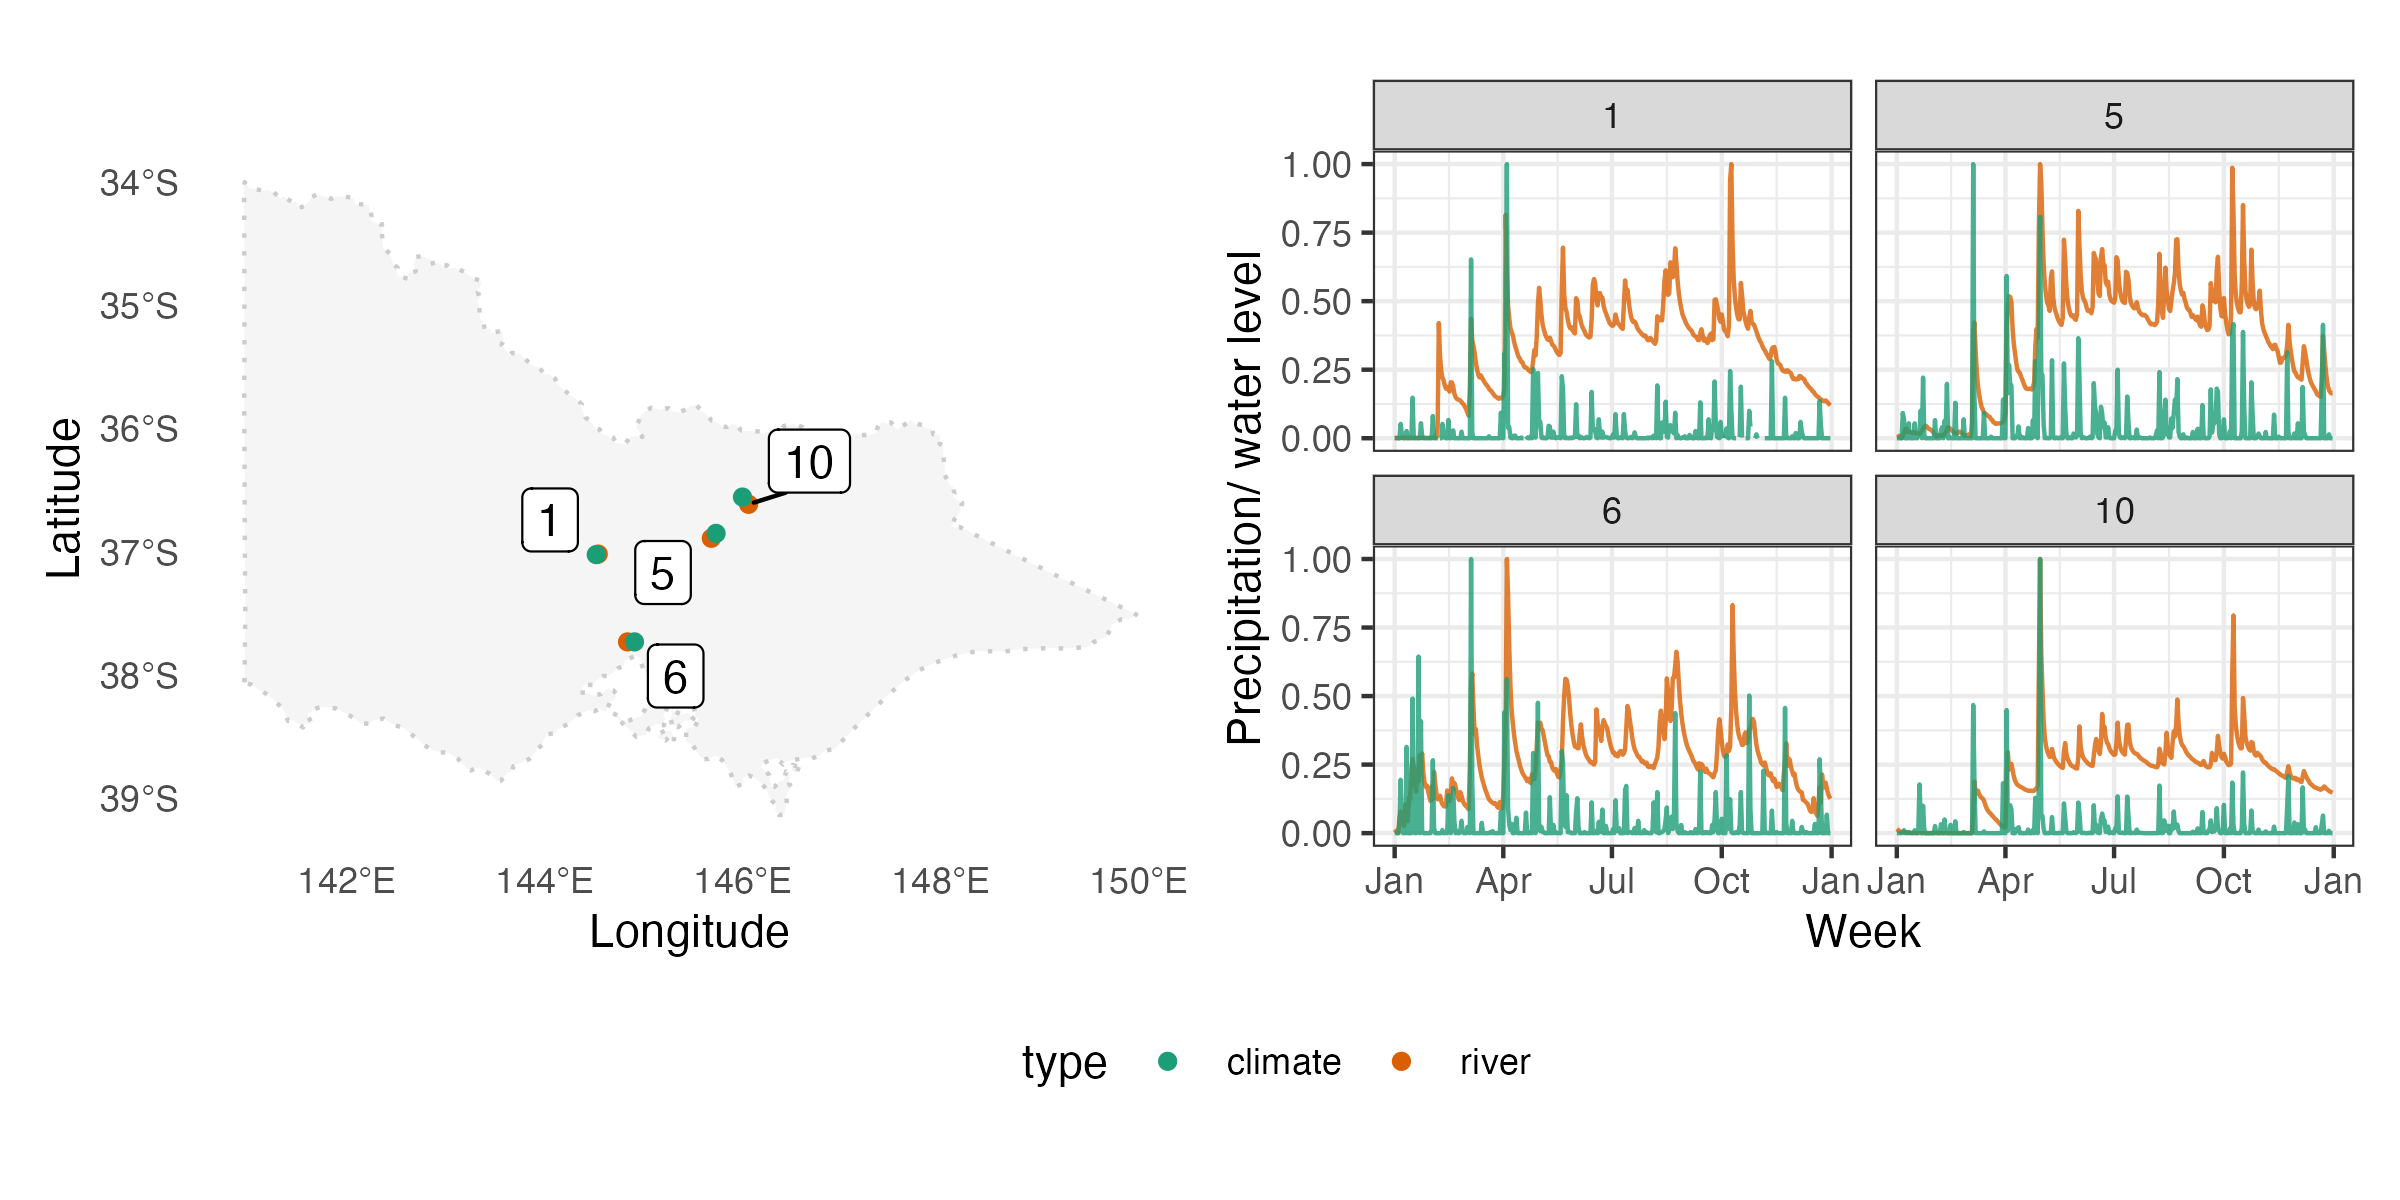
\includegraphics[width=1\linewidth]{/Users/sherryzhang/Documents/research/paper-cubble/figures/matching} \caption{Matched weather stations and river gauges on the map (A) and across time (B). Precipitation and water level have been standardised between 0 and 1 to be displayed on the same scale. The increases in the precipitation is reflected by the water level.}\label{fig:matching}
\end{figure}

\hypertarget{era5-climate-reanalysis-data}{%
\subsection{ERA5: climate reanalysis
data}\label{era5-climate-reanalysis-data}}

ERA5 data (\protect\hyperlink{ref-hersbach2020era5}{Hersbach et al.
2020}) is the latest reanalysis of global atmosphere, land surface, and
ocean waves from 1950 onwards and is available in the NetCDF format from
European Centre for Medium-Range Weather Forecasts (ECMWF). The data can
be directly downloaded from
\href{https://cds.climate.copernicus.eu/cdsapp\#!/dataset/reanalysis-era5-pressure-levels?tab=overview}{Copernicus
Climate Data Store (CDS)} website or programmatically via an R package
\pkg{ecmwfr} (\protect\hyperlink{ref-ecwmfr}{Hufkens, Stauffer, and
Campitelli 2019}). The \code{era5-pressure} data contains variable
\emph{specific humidity} and \emph{geopotential} on the 10 hPa pressure
level on four dates: 2002-09-22, 2002-09-26, 2002-09-30, and 2002-10-04.
Once downloaded, the data can be read into a cubble as:

\begin{Shaded}
\begin{Highlighting}[]
\NormalTok{raw }\OtherTok{\textless{}{-}}\NormalTok{ ncdf4}\SpecialCharTok{::}\FunctionTok{nc\_open}\NormalTok{(here}\SpecialCharTok{::}\FunctionTok{here}\NormalTok{(}\StringTok{"data/era5{-}pressure.nc"}\NormalTok{))}
\NormalTok{dt }\OtherTok{\textless{}{-}} \FunctionTok{as\_cubble}\NormalTok{(raw, }\AttributeTok{vars =} \FunctionTok{c}\NormalTok{(}\StringTok{"q"}\NormalTok{, }\StringTok{"z"}\NormalTok{))}
\end{Highlighting}
\end{Shaded}

Figure \ref{fig:netcdf} reproduces the ERA5 data row of Figure 19 in
Hersbach et al. (\protect\hyperlink{ref-hersbach2020era5}{2020}). It
shows the southern polar vortex splits into two on 2002-09-26 and
further splits into four on 2002-10-04 in the stratosphere. Readers
interested in the analysis of this figure can refer to Hersbach et al.
(\protect\hyperlink{ref-hersbach2020era5}{2020}), Simmons et al.
(\protect\hyperlink{ref-simmons2020global}{2020}) and Simmons et al.
(\protect\hyperlink{ref-simmons2005ecmwf}{2005}) for more details.

\begin{figure}
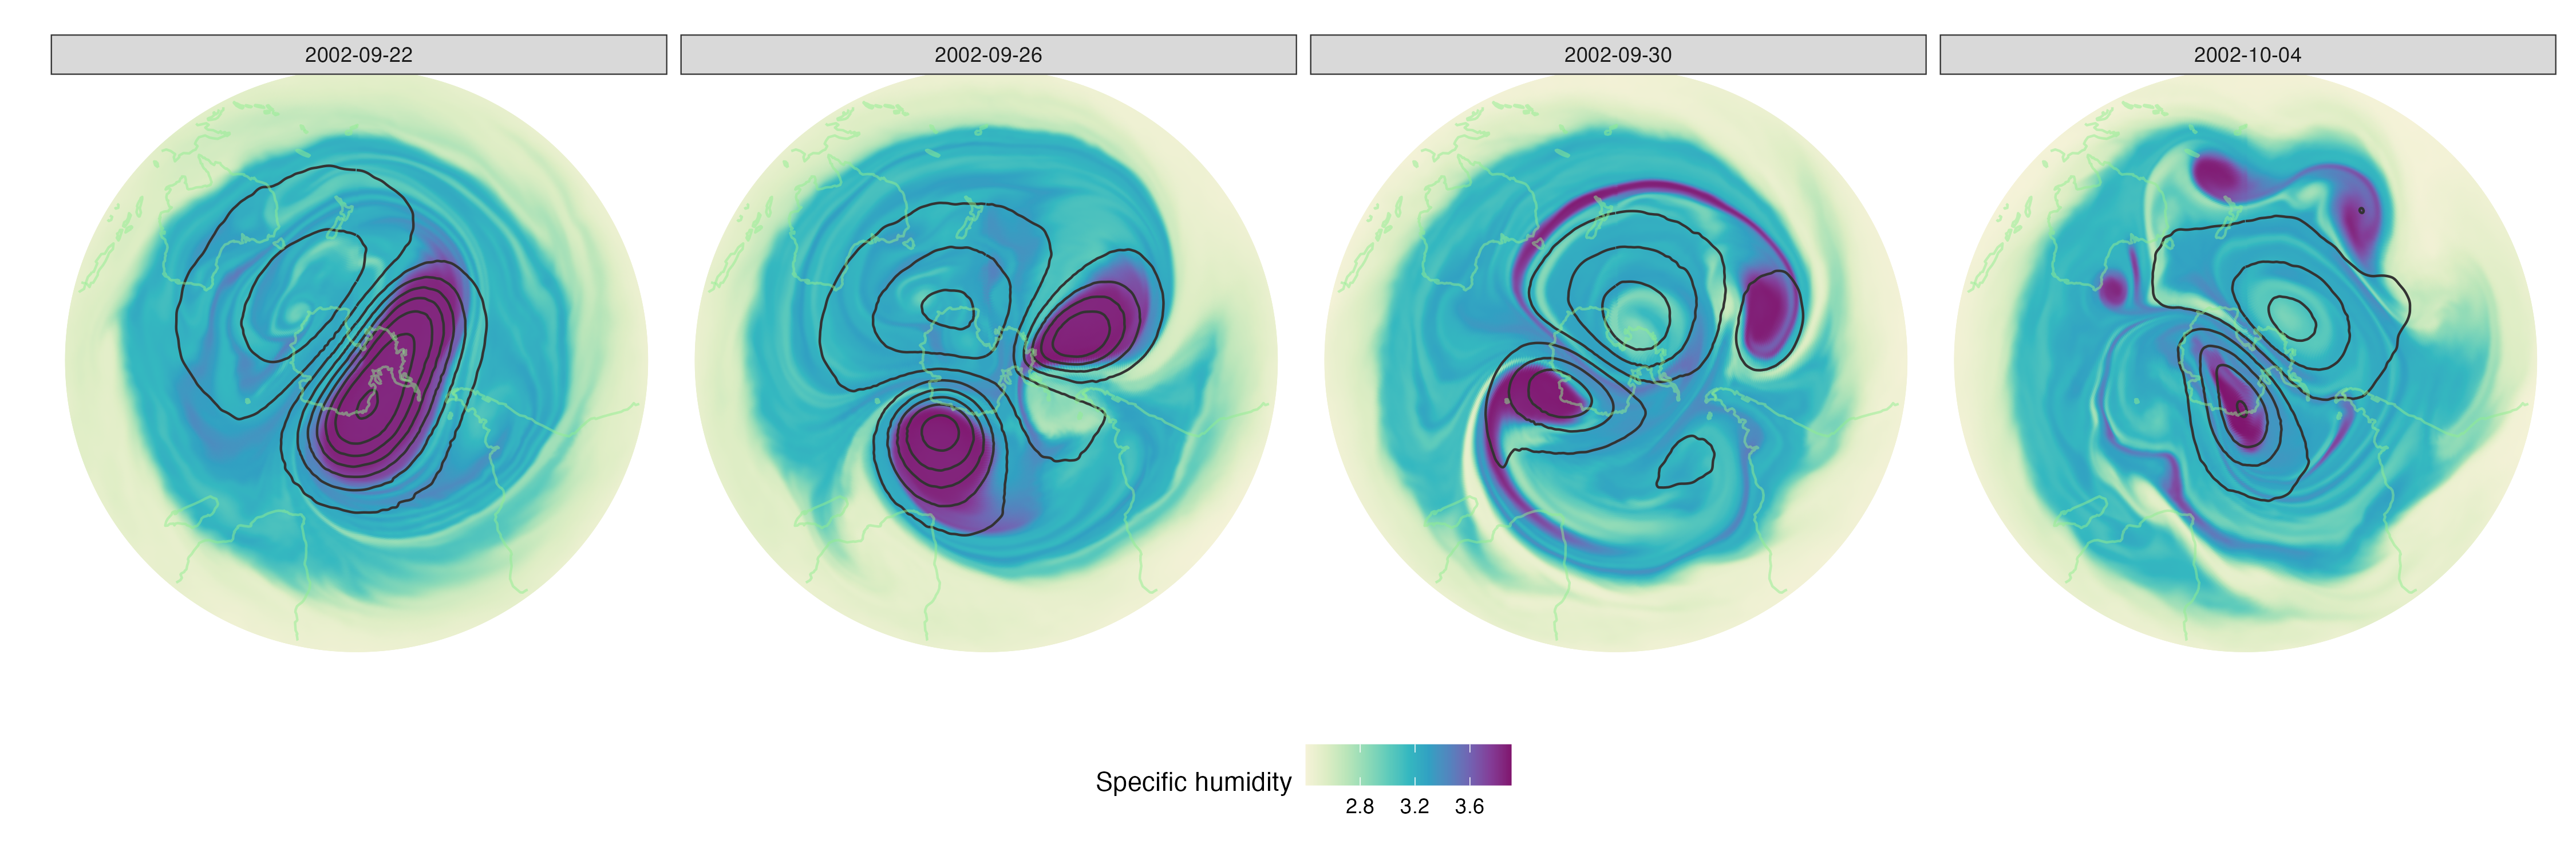
\includegraphics[width=1\linewidth]{/Users/sherryzhang/Documents/research/paper-cubble/figures/netcdf} \caption{A reproduction of the second row (ERA5 data) of Figure 19 in  Hersbach et al (2020).}\label{fig:netcdf}
\end{figure}

\hypertarget{interative-graphic}{%
\subsection{Interative graphic}\label{interative-graphic}}

With spatio-temporal data, users may wish to make plots to learn the
spatial distribution of a variable, or to find patterns, such as trend
or seasonality, in the time series. Combining this two types of plot
with interactivity let users to link between points on the map and the
corresponding time series to explore the spatial and temporal dimension
of the data simultaneously. Below is an example that describes the
process of building an interactive graphic with \pkg{cubble} and
\pkg{crosstalk} The example explores the variation of monthly
temperature range with \code{weatherdata::climate_full} data.

The temperature range is calculated as the difference between
\code{tmax} and \code{tmin} and its monthly average over 2016 - 2020 is
taken before calculating the variance. A \code{SharedData} object is
constructed for each form of the cubble and the same \code{group}
argument ensures the cross-linking of the two forms via the common
\code{id} column. The spatial map and time series plot are then made
with each \code{SharedData} objects separately. In this example,
stations on the Australia map, made from the nested form, are coloured
by the calculated variance and a ribbon band is constructed using the
long form cubble to show the maximum and minimum temperature of each
station across month. With a different dataset, users are free to
calculate any per station measure in the nested form or to make any
time-wise summary of the data in the long form to customise the spatial
or temporal view. The cross-linking between the two plots is always
safeguarded by the shared \code{id} column embedded in the cubble
structure. Below is the pseudo code that outlines the process to
construct an interactive graphic described above:

\begin{Shaded}
\begin{Highlighting}[]
\CommentTok{\# data pre{-}processing}
\NormalTok{clean }\OtherTok{\textless{}{-}}\NormalTok{ weatherdata}\SpecialCharTok{::}\NormalTok{climate\_full }\SpecialCharTok{|}\ErrorTok{\textgreater{}}\NormalTok{ ...}

\CommentTok{\# created SharedData instance for crosstalk}
\NormalTok{nested }\OtherTok{\textless{}{-}}\NormalTok{ clean }\SpecialCharTok{|}\ErrorTok{\textgreater{}}\NormalTok{ SharedData}\SpecialCharTok{$}\FunctionTok{new}\NormalTok{(}\SpecialCharTok{\textasciitilde{}}\NormalTok{id, }\AttributeTok{group =} \StringTok{"cubble"}\NormalTok{)}
\NormalTok{long }\OtherTok{\textless{}{-}} \FunctionTok{face\_temporal}\NormalTok{(clean) }\SpecialCharTok{|}\ErrorTok{\textgreater{}}\NormalTok{ SharedData}\SpecialCharTok{$}\FunctionTok{new}\NormalTok{(}\SpecialCharTok{\textasciitilde{}}\NormalTok{id, }\AttributeTok{group =} \StringTok{"cubble"}\NormalTok{)}

\CommentTok{\# create the spatial and temporal view each with a ShareData instance}
\NormalTok{p1 }\OtherTok{\textless{}{-}}\NormalTok{ nested }\SpecialCharTok{|}\ErrorTok{\textgreater{}}\NormalTok{ ...}
\NormalTok{p2 }\OtherTok{\textless{}{-}}\NormalTok{ long }\SpecialCharTok{|}\ErrorTok{\textgreater{}}\NormalTok{ ...}

\CommentTok{\# Combine p1 and p2}
\NormalTok{crosstalk}\SpecialCharTok{::}\FunctionTok{bscols}\NormalTok{(plotly}\SpecialCharTok{::}\FunctionTok{ggplotly}\NormalTok{(p1), plotly}\SpecialCharTok{::}\FunctionTok{ggplotly}\NormalTok{(p2), ...)}
\end{Highlighting}
\end{Shaded}

In Figure \ref{fig:interactive-linking}, the first row shows the initial
view of the interactive graphic. On the map, most regions in Australia
have low variance of temperature range while the north-west coastline,
bottom of South Australia, and Victoria stands out with larger monthly
changes. In the second row, Mount Elizabeth is selected on the map given
its high variance colour on the initial map and this links to the ribbon
on the right. The third row the lowest temperature in August and this
corresponds to Thredbo AWS in the Victoria and New South Wales border.
Another station in the Tasmania island is selected on the map to cross
compare with Thredbo AWS.

\begin{figure}
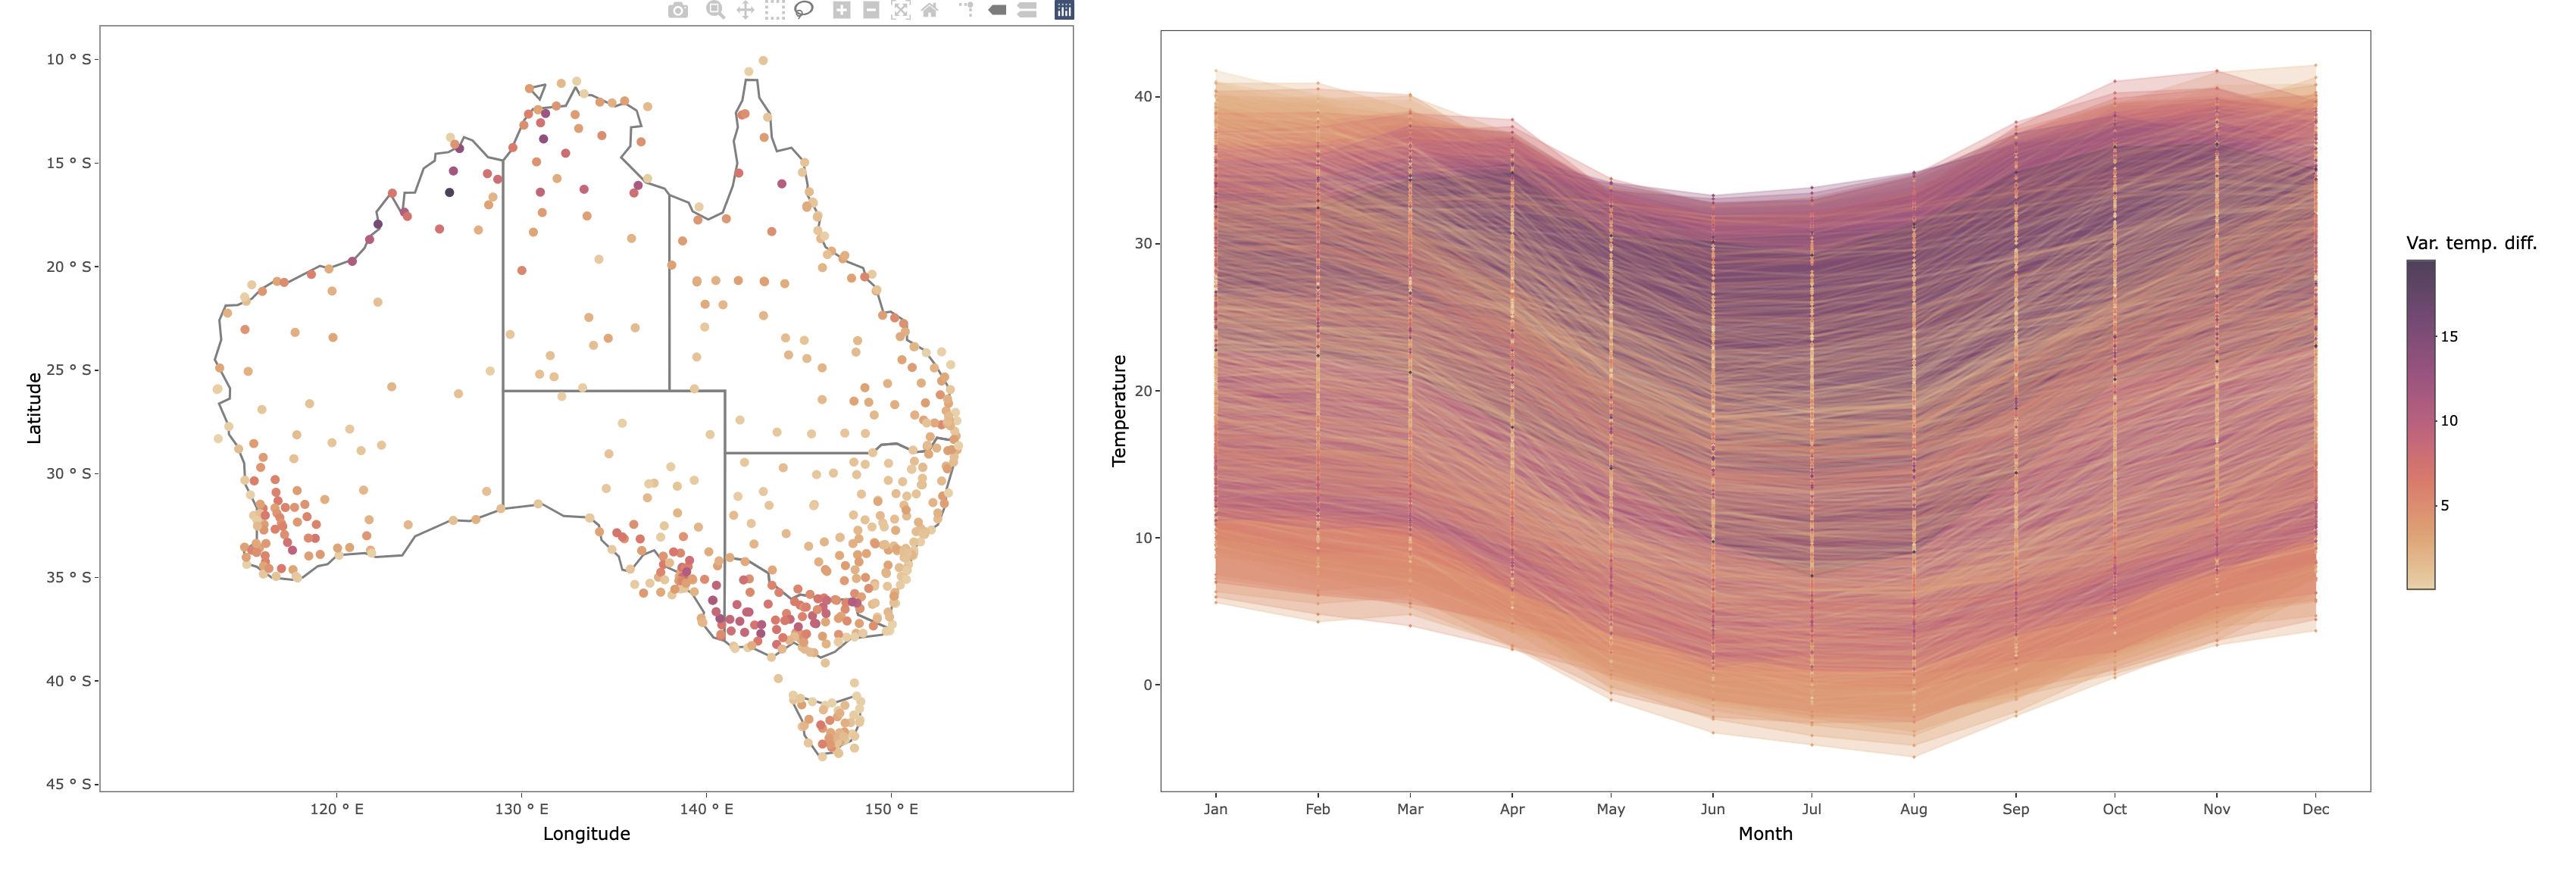
\includegraphics[width=1\linewidth,height=0.23\textheight]{/Users/sherryzhang/Documents/research/paper-cubble/figures/linking} 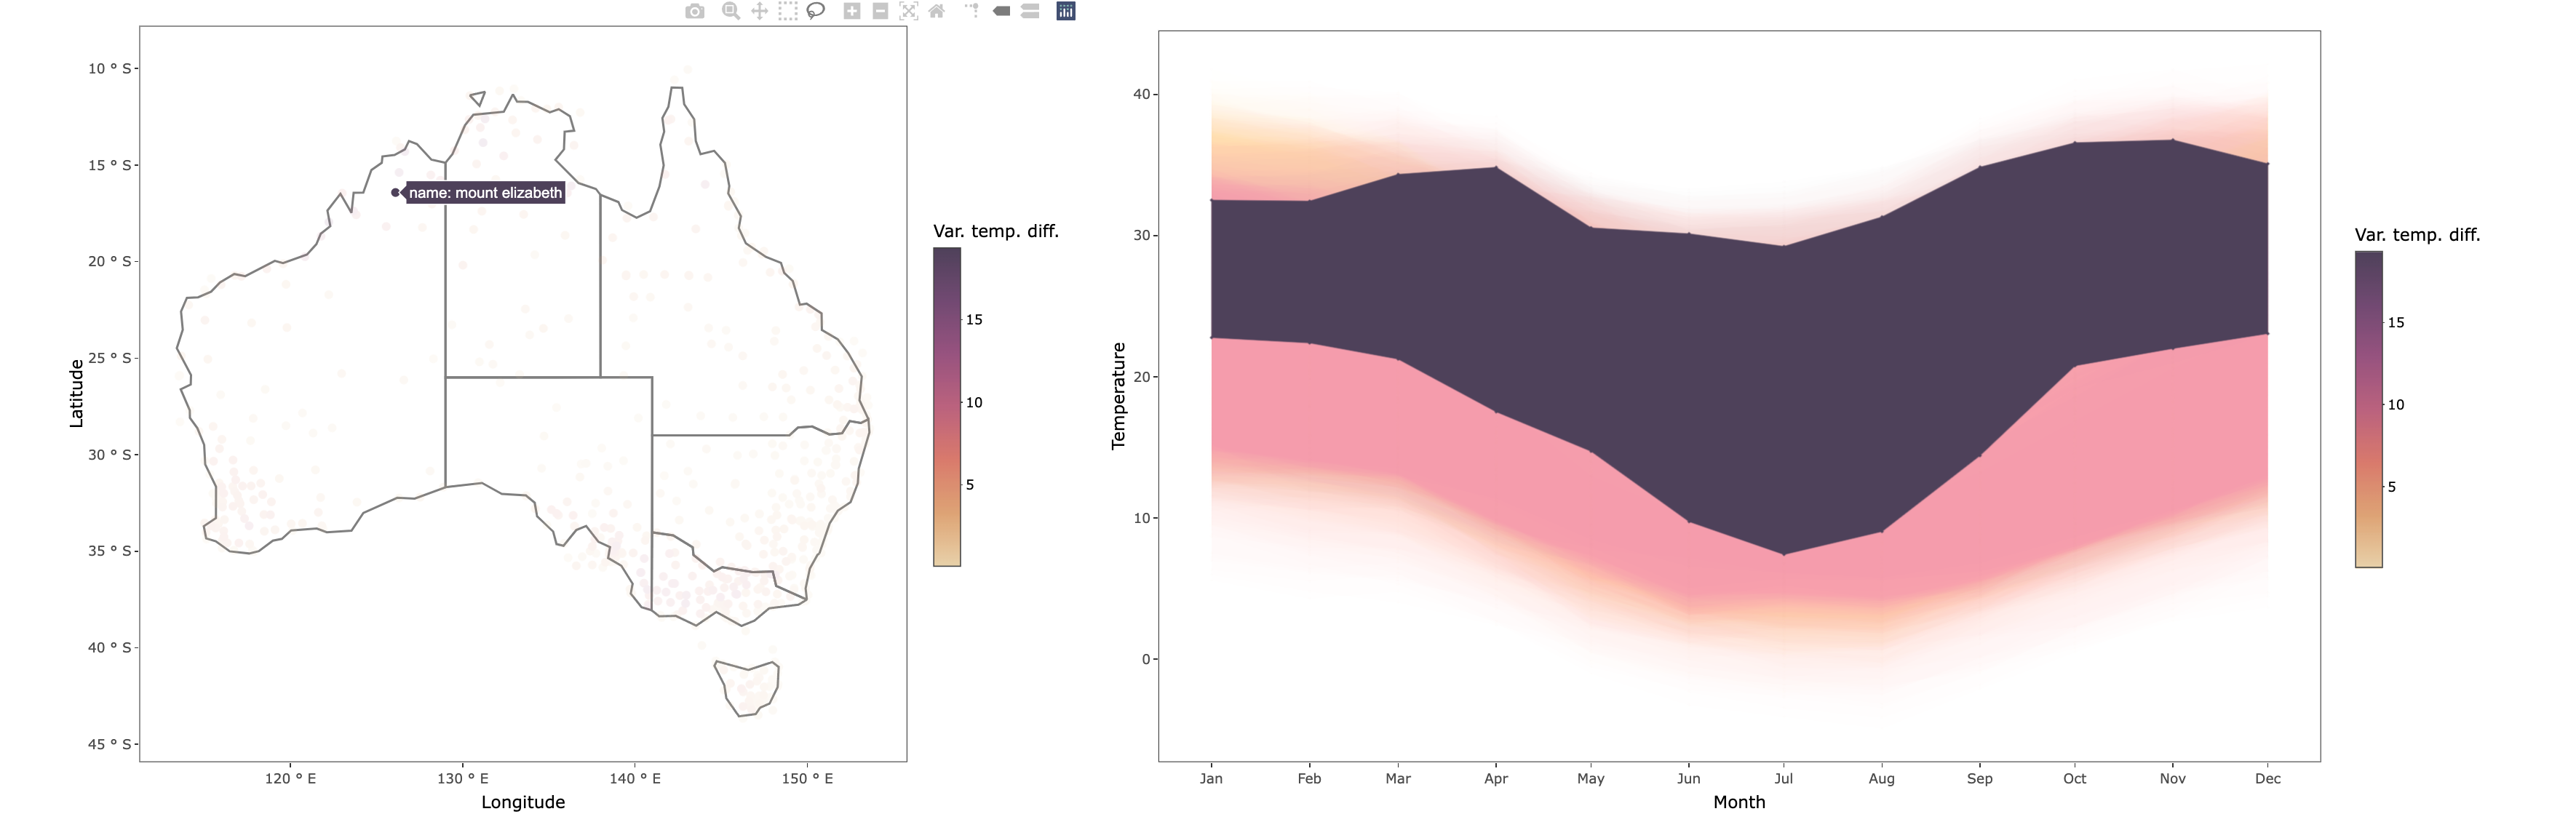
\includegraphics[width=1\linewidth,height=0.23\textheight]{/Users/sherryzhang/Documents/research/paper-cubble/figures/linking-north} 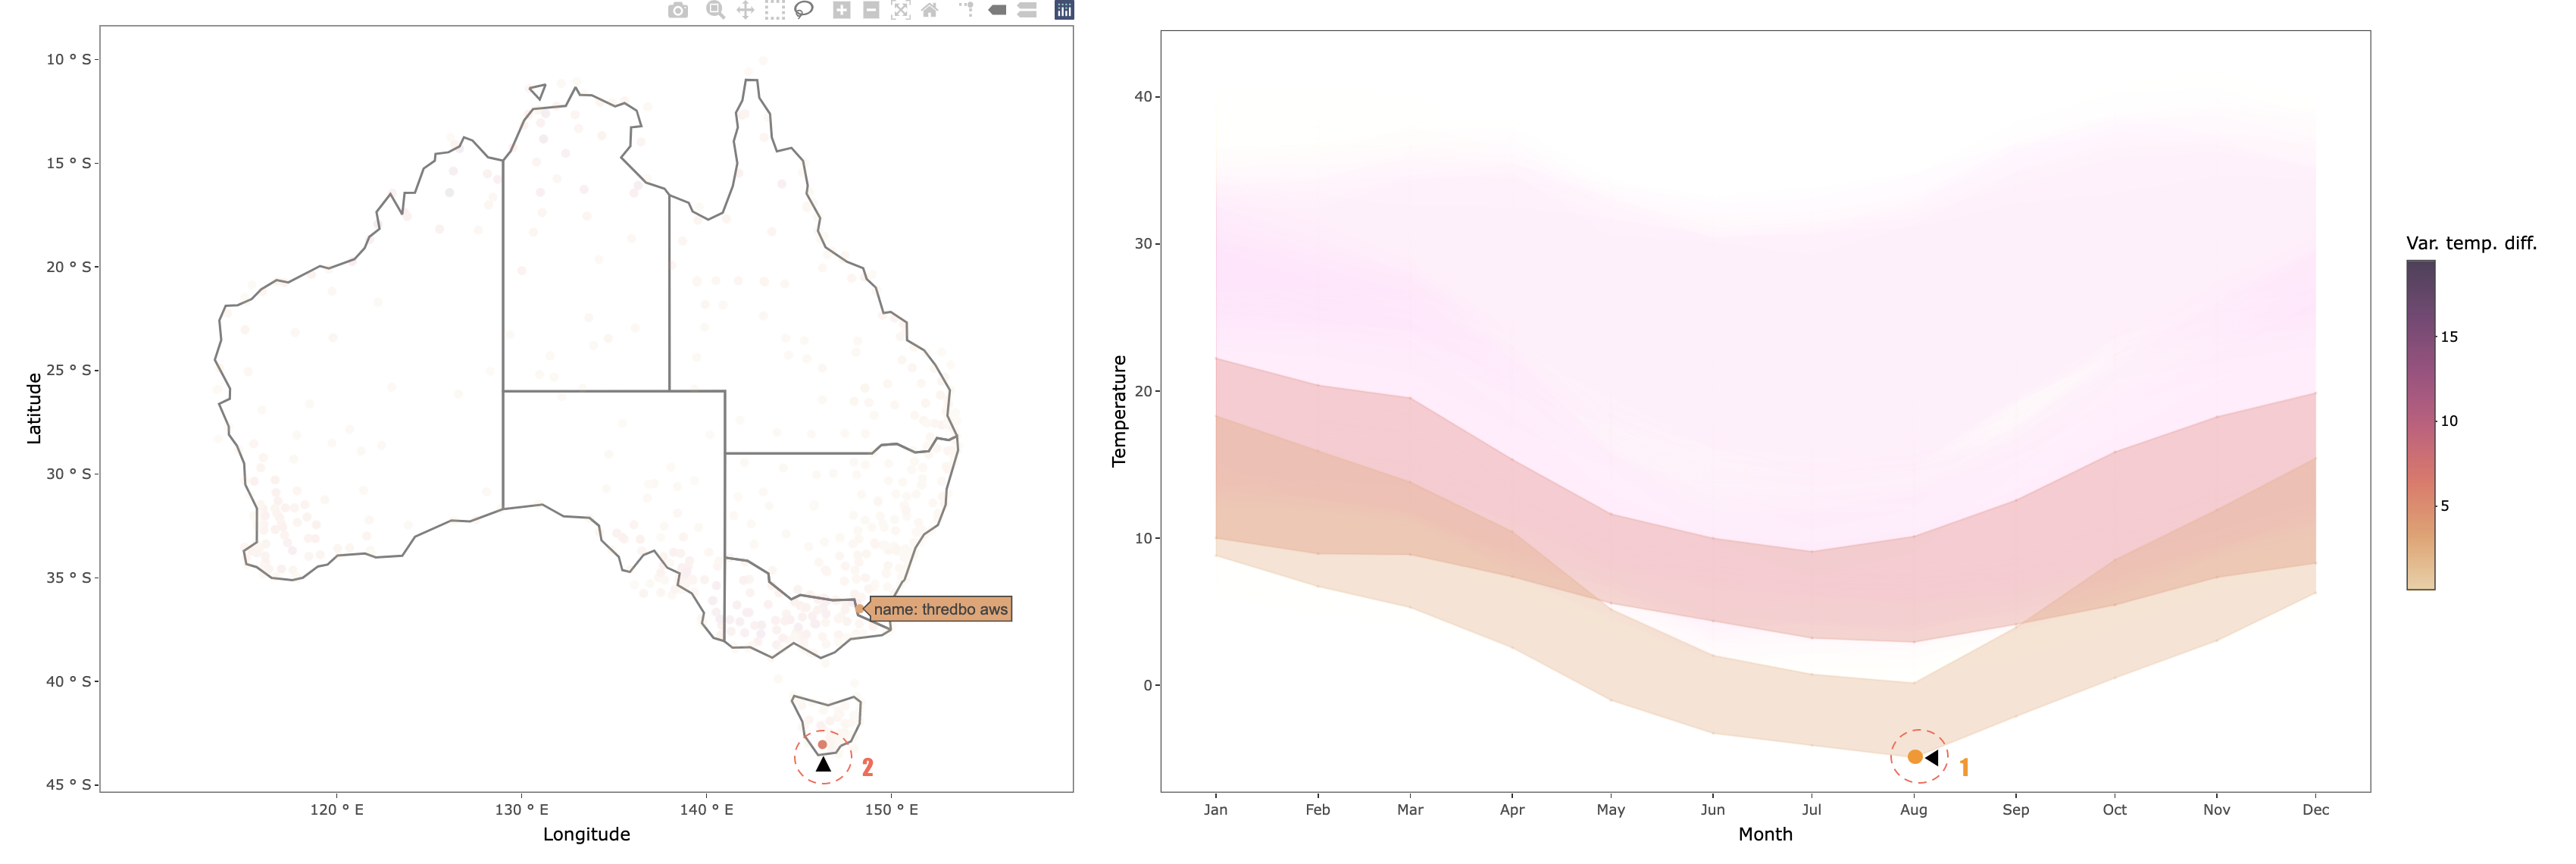
\includegraphics[width=1\linewidth,height=0.23\textheight]{/Users/sherryzhang/Documents/research/paper-cubble/figures/linking-lower} \caption{Exploring temperature variation using linking of a map and seasonal display. Each row is a screen dump of the process. The top row shows all locations and all temperature profiles. Selecting a location with high variance on the map produces the plot in the second row. The maximum nad minimum temperature is shown using a ribbon. The bottom row first selects the lowest temperature in Auguest in the seasonal display. A location in the Tasmania Island is then selected to compare the temperature variation with Thredbo AWS.}\label{fig:interactive-linking}
\end{figure}

This plot can also be made using \pkg{cubble} and \pkg{leaflet} where
the temperature range can be displayed as a small subplot upon clicking
on the map. This would require first creating the popup plots from the
long form cubble as a vector and then add these plots to a leaflet map
created from the nested cubble, with \code{leafpop::addPopupGraphs()}:

\begin{Shaded}
\begin{Highlighting}[]
\CommentTok{\# data pre{-}processing}
\NormalTok{clean }\OtherTok{\textless{}{-}}\NormalTok{ weatherdata}\SpecialCharTok{::}\NormalTok{climate\_full }\SpecialCharTok{|}\ErrorTok{\textgreater{}}\NormalTok{ ...}

\CommentTok{\# use the long form to create subplots for each station}
\NormalTok{df\_id }\OtherTok{\textless{}{-}} \FunctionTok{unique}\NormalTok{(clean}\SpecialCharTok{$}\NormalTok{id)}
\NormalTok{p }\OtherTok{\textless{}{-}} \FunctionTok{map}\NormalTok{(}\DecValTok{1}\SpecialCharTok{:}\FunctionTok{length}\NormalTok{(df\_id), }\ControlFlowTok{function}\NormalTok{(i)\{}
\NormalTok{  dt }\OtherTok{\textless{}{-}}\NormalTok{ clean }\SpecialCharTok{|}\ErrorTok{\textgreater{}} \FunctionTok{filter}\NormalTok{(id }\SpecialCharTok{==}\NormalTok{ df\_id[i])}
  \FunctionTok{ggplot}\NormalTok{(dt) }\SpecialCharTok{|}\ErrorTok{\textgreater{}}\NormalTok{ ...}
\NormalTok{\})}

\CommentTok{\# create nested form leaflet map with temperature band as subplots}
\NormalTok{nested }\OtherTok{\textless{}{-}} \FunctionTok{face\_spatial}\NormalTok{(clean)}
\FunctionTok{leaflet}\NormalTok{(nested) }\SpecialCharTok{|}\ErrorTok{\textgreater{}}
  \FunctionTok{addTiles}\NormalTok{() }\SpecialCharTok{|}\ErrorTok{\textgreater{}}
  \FunctionTok{addCircleMarkers}\NormalTok{(}\AttributeTok{group =} \StringTok{"a"}\NormalTok{, ...) }\SpecialCharTok{|}\ErrorTok{\textgreater{}}
\NormalTok{  leafpop}\SpecialCharTok{::}\FunctionTok{addPopupGraphs}\NormalTok{(}\AttributeTok{graph =}\NormalTok{ p, ...)}
\end{Highlighting}
\end{Shaded}

Figure \ref{fig:interactive-popup} shows Figure
\ref{fig:interactive-linking} made made with leaflet and popups
(\protect\hyperlink{ref-leafpop}{Appelhans and Detsch 2021}).

\begin{figure}
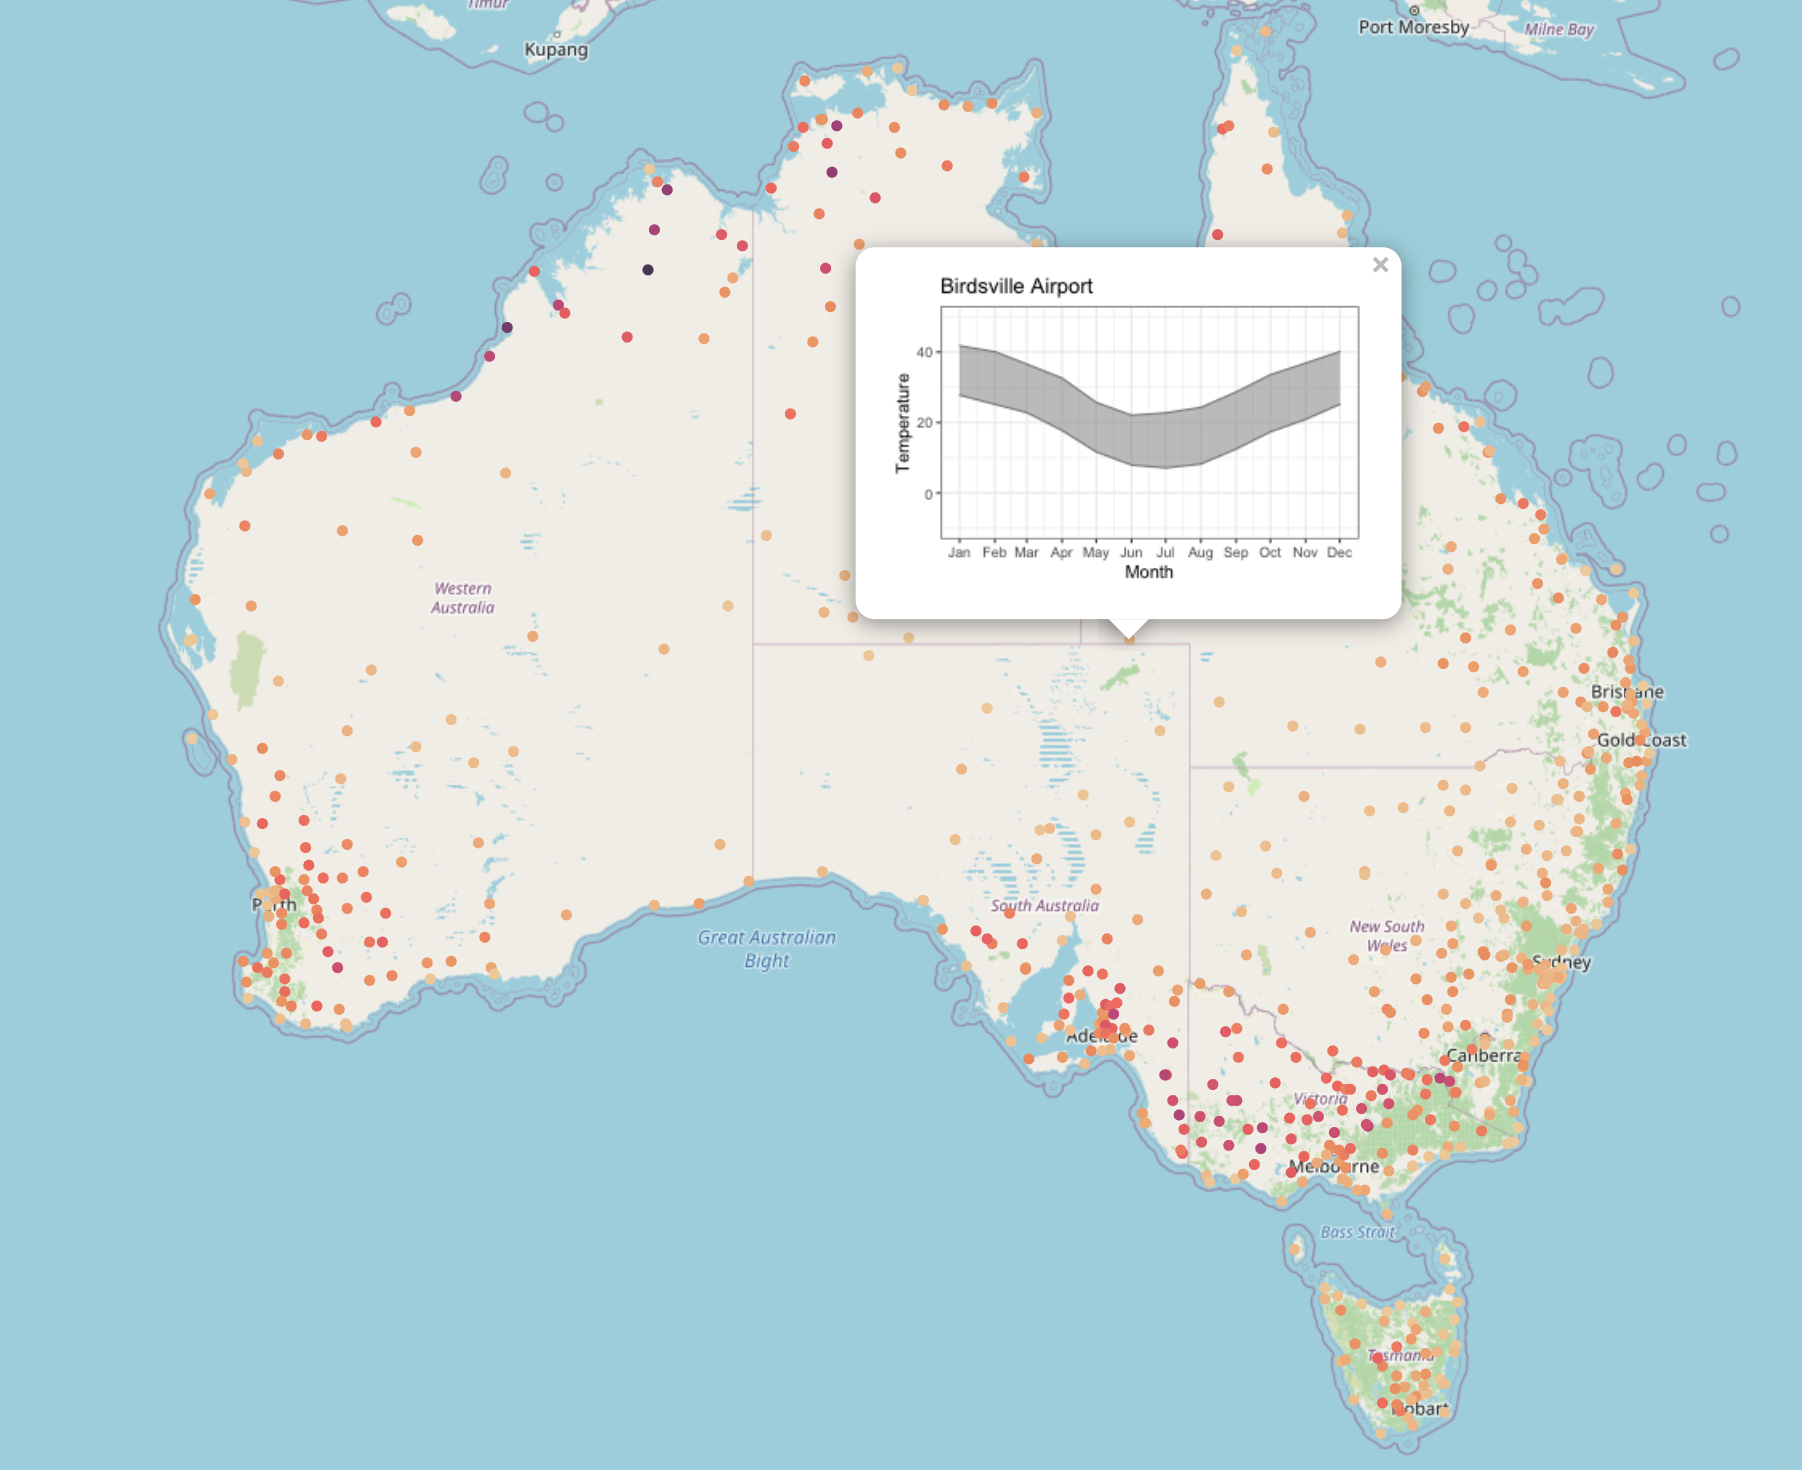
\includegraphics[width=0.45\linewidth,height=0.25\textheight]{/Users/sherryzhang/Documents/research/paper-cubble/figures/popup-mid} \caption{Same as Figure 11 with thetemperature variation shown as a popup in the leaflet map.}\label{fig:interactive-popup}
\end{figure}

\hypertarget{conclusion}{%
\section{Conclusion}\label{conclusion}}

This paper describes an \proglang{R} package \pkg{cubble} for
manipulating and visualising spatio-temporal data. A new data structure,
\code{cubble} that builds from the \code{rowwise_df} and
\code{grouped_df} class in the tidyverse ecosystem, is proposed to
connect the time invariant and varying variables in the spatio-temporal
data. This design frees the data analysts from spending time on
organising variables of different observational units. The data
structure is also flexible to the techniques and packages analysts use
to analyse the data, for example, in the matching example in section
4.3, users are free to use algorithms from another package to cluster
stations.

Further development and maintenance of the package involves responding
to changes in the tidyverse packages that \pkg{cubble} imports, in
particular, \pkg{tibble}, \pkg{tidyr}, and \pkg{dplyr}. Another area for
further development is to extend \pkg{cubble} to other spatial objects
other than points.

\newpage

\hypertarget{acknowledgement}{%
\section{Acknowledgement}\label{acknowledgement}}

This work is funded by the Commonwealth Scientific and Industrial
Research Organisation (CSIRO) Data61 Scholarship and started while
Nicolas Langrené was affiliated with CSIRO's Data61. The article is
created using \pkg{knitr} (\protect\hyperlink{ref-knitr}{Xie 2015}) and
\pkg{rmarkdown} (\protect\hyperlink{ref-rmarkdown}{Xie, Allaire, and
Grolemund 2018}) in R. The source code for reproducing this paper can be
found at: \url{https://github.com/huizezhang-sherry/paper-cubble}.

\hypertarget{appendix}{%
\section{Appendix}\label{appendix}}

\begin{figure}

{\centering 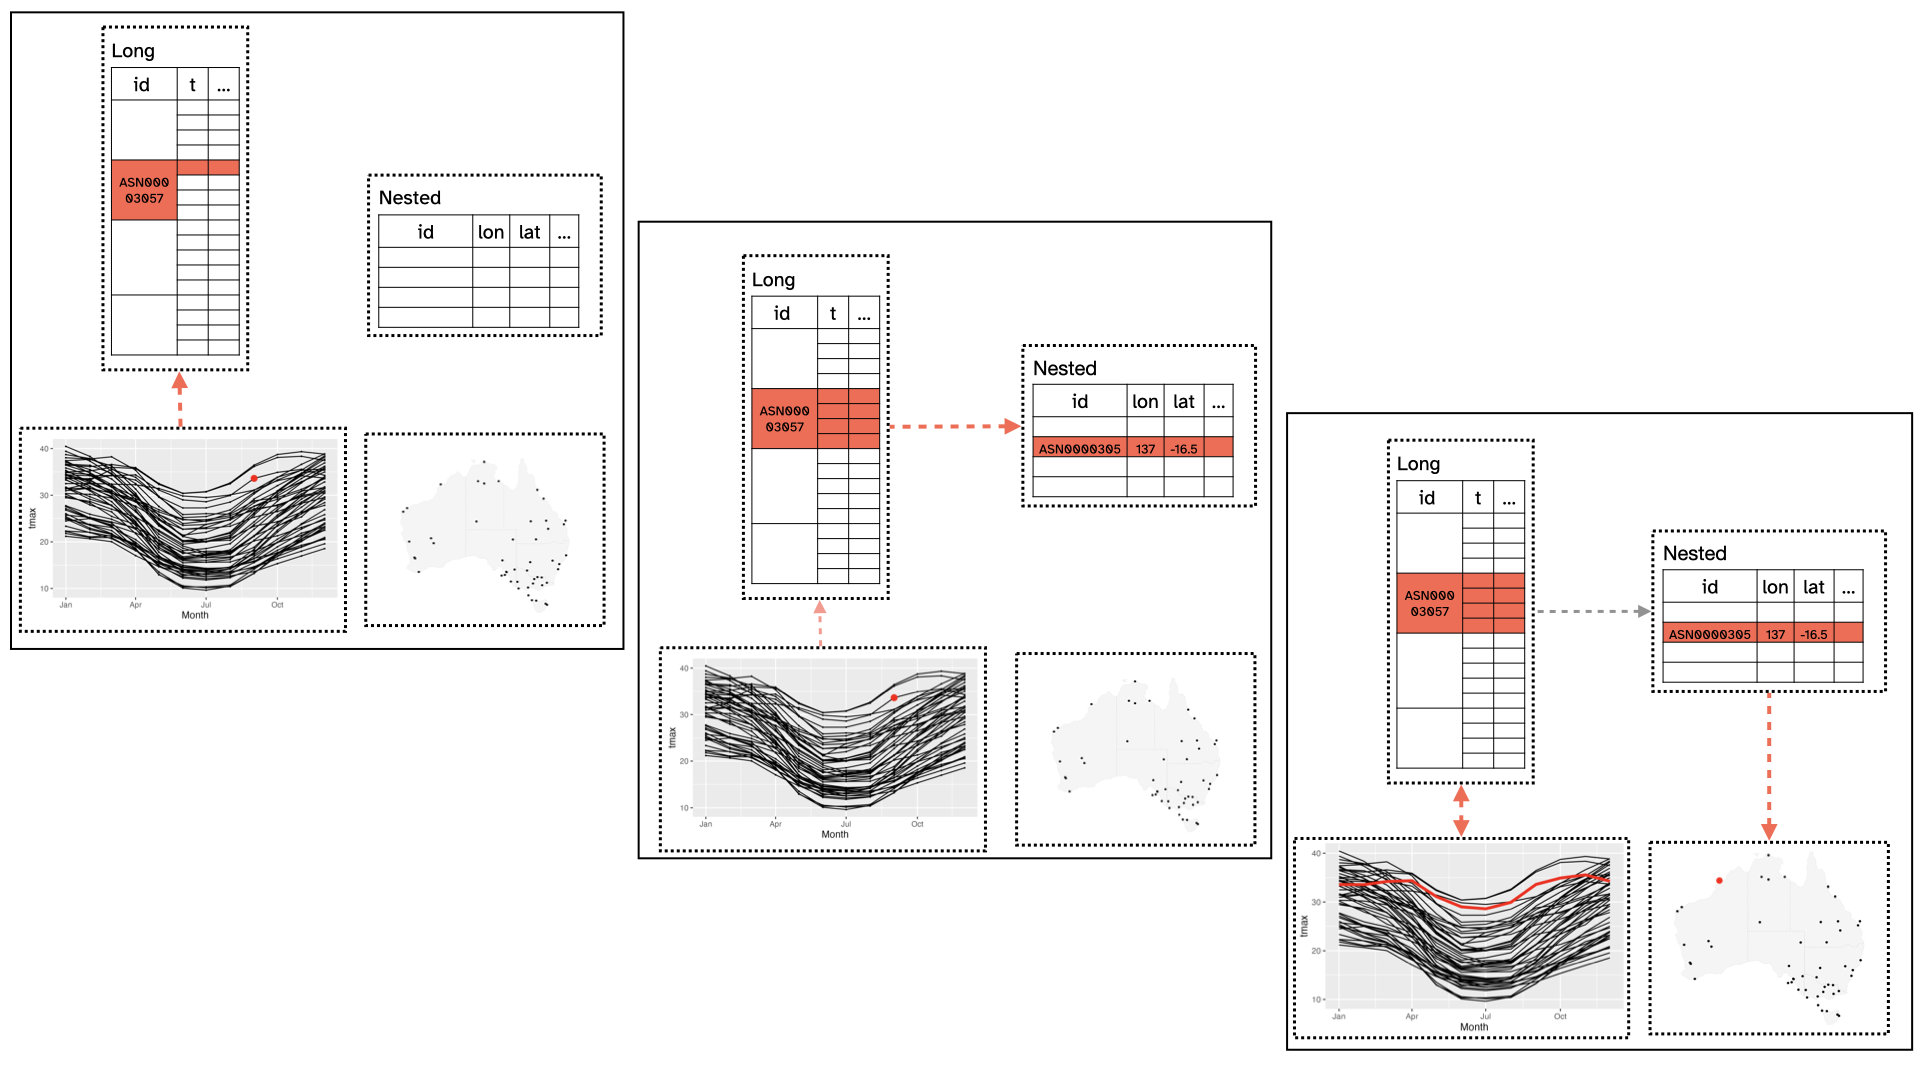
\includegraphics[width=1\linewidth,height=0.4\textheight]{/Users/sherryzhang/Documents/research/paper-cubble/figures/diagram-keynotes/diagram-keynotes.005} 

}

\caption{An illustration of the data model under interactive graphics with cubble. When a point on the time series is selected, the corresponding row in the long cubble will be activated. This will link to all the rows with the same id in the long cubble and the row in the nested cubble with the smae id (middle). Both plots will be updated with the full line selected and the point highlighted on the map (right).}\label{fig:illu-interactive-2}
\end{figure}

\newpage

\hypertarget{refs}{}
\begin{CSLReferences}{1}{0}
\leavevmode\vadjust pre{\hypertarget{ref-leafpop}{}}%
Appelhans, Tim, and Florian Detsch. 2021. \emph{\pkg{leafpop}: Include
Tables, Images and Graphs in Leaflet Pop-Ups}.
\url{https://CRAN.R-project.org/package=leafpop}.

\leavevmode\vadjust pre{\hypertarget{ref-bach_review_2014}{}}%
Bach, Benjamin, Pierre Dragicevic, Dragicevic Archambault, Christophe
Hurter, and Sheelagh Carpendale. 2014. {``A {Review} of {Temporal}
{Data} {Visualizations} {Based} on {Space}-{Time} {Cube}
{Operations}.''} \emph{Eurographics Conference on Visualization}, 19.
\url{https://hal.inria.fr/hal-01006140/}.

\leavevmode\vadjust pre{\hypertarget{ref-buja1988elements}{}}%
Buja, Andreas, Daniel Asimov, and Catherine Hurley. 1988. {``Elements of
a Viewing Pipeline.''} \emph{Dynamic Graphics Statistics}, 277.

\leavevmode\vadjust pre{\hypertarget{ref-buja1996interactive}{}}%
Buja, Andreas, Dianne Cook, and Deborah F Swayne. 1996. {``Interactive
High-Dimensional Data Visualization.''} \emph{Journal of Computational
and Graphical Statistics} 5 (1): 78--99.
\url{https://doi.org/10.2307/1390754}.

\leavevmode\vadjust pre{\hypertarget{ref-cheng2016enabling}{}}%
Cheng, Xiaoyue, Dianne Cook, and Heike Hofmann. 2016. {``Enabling
Interactivity on Displays of Multivariate Time Series and Longitudinal
Data.''} \emph{Journal of Computational and Graphical Statistics} 25
(4): 1057--76. \url{https://doi.org/10.1080/10618600.2015.1105749}.

\leavevmode\vadjust pre{\hypertarget{ref-cocchi2019data}{}}%
Cocchi, Marina. 2019. \emph{Data Fusion Methodology and Applications}.
Elsevier.

\leavevmode\vadjust pre{\hypertarget{ref-hersbach2020era5}{}}%
Hersbach, Hans, Bill Bell, Paul Berrisford, Shoji Hirahara, András
Horányi, Joaquín Muñoz-Sabater, Julien Nicolas, et al. 2020. {``The Era5
Global Reanalysis.''} \emph{Quarterly Journal of the Royal
Meteorological Society} 146 (730): 1999--2049.

\leavevmode\vadjust pre{\hypertarget{ref-ecwmfr}{}}%
Hufkens, Koen, Reto Stauffer, and Elio Campitelli. 2019. {``The
\pkg{ecwmfr} Package: An Interface to ECMWF API Endpoints.''}
\url{https://doi.org/10.5281/zenodo.2647541}.

\leavevmode\vadjust pre{\hypertarget{ref-jr_herring_opengis_2011}{}}%
J.R. Herring. 2011. {``{OpenGIS}® {Implementation} {Standard} for
{Geographic} Information - {Simple} Feature Access - {Part} 1: {Common}
Architecture.''} Open Geospatial Consortium Inc.
\href{http://portal.\%20opengeospatial.org/files/?artifact_id=25355}{http://portal.
opengeospatial.org/files/?artifact\_id=25355}.

\leavevmode\vadjust pre{\hypertarget{ref-lu_multidimensional_2018}{}}%
Lu, Meng, Marius Appel, and Edzer Pebesma. 2018. {``Multidimensional
{Arrays} for {Analysing} {Geoscientific} {Data}.''} \emph{ISPRS
International Journal of Geo-Information} 7 (8): 313.
\url{https://doi.org/10.3390/ijgi7080313}.

\leavevmode\vadjust pre{\hypertarget{ref-mcintosh2018using}{}}%
McIntosh, Avery I, Helen E Jenkins, Laura F White, Marinus Barnard, Dana
R Thomson, Tania Dolby, John Simpson, et al. 2018. {``Using Routinely
Collected Laboratory Data to Identify High Rifampicin-Resistant
Tuberculosis Burden Communities in the Western Cape Province, South
Africa: A Retrospective Spatiotemporal Analysis.''} \emph{PLoS Medicine}
15 (8): e1002638.

\leavevmode\vadjust pre{\hypertarget{ref-michna2013rnetcdf}{}}%
Michna, Pavel, and Milton Woods. 2013. {``\pkg{RNetCDF}: A Package for
Reading and Writing NetCDF Datasets.''} \emph{The R Journal} 5 (2):
29--36.

\leavevmode\vadjust pre{\hypertarget{ref-rnetcdf}{}}%
---------. 2021. \emph{\pkg{RNetCDF}: Interface to 'NetCDF' Datasets}.
\url{https://CRAN.R-project.org/package=RNetCDF}.

\leavevmode\vadjust pre{\hypertarget{ref-tibble}{}}%
Müller, Kirill, and Hadley Wickham. 2021. \emph{Tibble: Simple Data
Frames}. \url{https://CRAN.R-project.org/package=tibble}.

\leavevmode\vadjust pre{\hypertarget{ref-spacetime}{}}%
Pebesma, Edzer. 2012. {``\pkg{spacetime}: Spatio-Temporal Data in r.''}
\emph{Journal of Statistical Software} 51 (7): 1--30.
\url{https://doi.org/10.18637/jss.v051.i07}.

\leavevmode\vadjust pre{\hypertarget{ref-stars}{}}%
---------. 2021. \emph{\pkg{stars}: Spatiotemporal Arrays, Raster and
Vector Data Cubes}. \url{https://CRAN.R-project.org/package=stars}.

\leavevmode\vadjust pre{\hypertarget{ref-sf}{}}%
Pebesma, Edzer J. 2018. {``Simple Features for \proglang{R}:
Standardized Support for Spatial Vector Data.''} \emph{R Journal} 10
(1): 439.

\leavevmode\vadjust pre{\hypertarget{ref-sp}{}}%
Pebesma, Edzer, and Roger S Bivand. 2005. {``S Classes and Methods for
Spatial Data: The \pkg{sp} Package.''} \emph{R News} 5 (2): 9--13.

\leavevmode\vadjust pre{\hypertarget{ref-ncdf4}{}}%
Pierce, David. 2019. \emph{\pkg{ncdf4}: Interface to Unidata netCDF
(Version 4 or Earlier) Format Data Files}.
\url{https://CRAN.R-project.org/package=ncdf4}.

\leavevmode\vadjust pre{\hypertarget{ref-xts}{}}%
Ryan, Jeffrey A., and Joshua M. Ulrich. 2020. \emph{\pkg{xts}:
eXtensible Time Series}. \url{https://CRAN.R-project.org/package=xts}.

\leavevmode\vadjust pre{\hypertarget{ref-simmons2005ecmwf}{}}%
Simmons, Adrian, Mariano Hortal, Graeme Kelly, Anthony McNally, Agathe
Untch, and Sakari Uppala. 2005. {``ECMWF Analyses and Forecasts of
Stratospheric Winter Polar Vortex Breakup: September 2002 in the
Southern Hemisphere and Related Events.''} \emph{Journal of the
Atmospheric Sciences} 62 (3): 668--89.
\url{https://doi.org/10.1175/JAS-3322.1}.

\leavevmode\vadjust pre{\hypertarget{ref-simmons2020global}{}}%
Simmons, Adrian, Cornel Soci, Julien Nicolas, Bill Bell, P. Berrisford,
Rossana Dragani, Johannes Flemming, et al. 2020. {``Global Stratospheric
Temperature Bias and Other Stratospheric Aspects of Era5 and Era5.1,''}
no. 859 (January). \url{https://doi.org/10.21957/rcxqfmg0}.

\leavevmode\vadjust pre{\hypertarget{ref-stuart2010matching}{}}%
Stuart, Elizabeth A. 2010. {``Matching Methods for Causal Inference: A
Review and a Look Forward.''} \emph{Statistical Science} 25 (1): 1.

\leavevmode\vadjust pre{\hypertarget{ref-tidync}{}}%
Sumner, Michael. 2020. \emph{\pkg{tidync}: A Tidy Approach to 'NetCDF'
Data Exploration and Extraction}.
\url{https://CRAN.R-project.org/package=tidync}.

\leavevmode\vadjust pre{\hypertarget{ref-sutherland2000orca}{}}%
Sutherland, Peter, Anthony Rossini, Thomas Lumley, Nicholas Lewin-Koh,
Julie Dickerson, Zach Cox, and Dianne Cook. 2000. {``\pkg{Orca}: A
Visualization Toolkit for High-Dimensional Data.''} \emph{Journal of
Computational and Graphical Statistics} 9 (3): 509--29.
\url{https://www.tandfonline.com/doi/abs/10.1080/10618600.2000.10474896}.

\leavevmode\vadjust pre{\hypertarget{ref-tsibble}{}}%
Wang, Earo, Dianne Cook, and Rob J Hyndman. 2020a. {``A New Tidy Data
Structure to Support Exploration and Modeling of Temporal Data.''}
\emph{Journal of Computational and Graphical Statistics} 29 (3):
466--78. \url{https://doi.org/10.1080/10618600.2019.1695624}.

\leavevmode\vadjust pre{\hypertarget{ref-wang2020calendar}{}}%
---------. 2020b. {``Calendar-Based Graphics for Visualizing People's
Daily Schedules.''} \emph{Journal of Computational and Graphical
Statistics} 29 (3): 490--502.

\leavevmode\vadjust pre{\hypertarget{ref-tidydata}{}}%
Wickham, Hadley. 2014. {``Tidy Data.''} \emph{Journal of Statistical
Software} 59 (10): 1--23. \url{https://doi.org/10.18637/jss.v059.i10}.

\leavevmode\vadjust pre{\hypertarget{ref-tidyverse}{}}%
Wickham, Hadley, Mara Averick, Jennifer Bryan, Winston Chang, Lucy
D'Agostino McGowan, Romain François, Garrett Grolemund, et al. 2019.
{``Welcome to the {tidyverse}.''} \emph{Journal of Open Source Software}
4 (43): 1686. \url{https://doi.org/10.21105/joss.01686}.

\leavevmode\vadjust pre{\hypertarget{ref-Wickham2012-yr}{}}%
Wickham, Hadley, Heike Hofmann, Charlotte Wickham, and Dianne Cook.
2012. {``Glyph-Maps for Visually Exploring Temporal Patterns in Climate
Data and Models.''} \emph{Environmetrics} 23 (5): 382--93.

\leavevmode\vadjust pre{\hypertarget{ref-knitr}{}}%
Xie, Yihui. 2015. \emph{Dynamic Documents with \proglang{R} and
\pkg{knitr}}. 2nd ed. Boca Raton, Florida: Chapman; Hall/CRC.
\url{https://yihui.name/knitr/}.

\leavevmode\vadjust pre{\hypertarget{ref-rmarkdown}{}}%
Xie, Yihui, J. J. Allaire, and Garrett Grolemund. 2018. \emph{R
Markdown: The Definitive Guide}. Boca Raton, Florida: Chapman; Hall/CRC.
\url{https://bookdown.org/yihui/rmarkdown}.

\leavevmode\vadjust pre{\hypertarget{ref-xie2014reactive}{}}%
Xie, Yihui, Heike Hofmann, and Xiaoyue Cheng. 2014. {``{Reactive
Programming for Interactive Graphics}.''} \emph{Statistical Science} 29
(2): 201--13. \url{https://doi.org/10.1214/14-STS477}.

\end{CSLReferences}

\bibliographystyle{unsrt}
\bibliography{../references.bib}


\end{document}
